\documentclass{report} 
\title{Appendix 2}
\date{Started 24 May 2024}
\author{Malcolm}
\usepackage{amsmath} %import math
\usepackage{mathtools} %more math
\usepackage{amssymb} %for QED symbol
\usepackage{amsthm} %
\usepackage{bm}%bold math
\usepackage{graphicx} %import imaging
\graphicspath{{./images/}} %set imaging path
\begin{document}
\maketitle

\tableofcontents

\appendix
\chapter{Differential Equations}
\section{First Order Differential Equations}
\subsection{Introduction to Ordinary Differential Equations\\(ODEs)} %030624
Here we introduce intuition for  Ordinary Differential Equations (ODEs) and introductory solving methods.\\
\vspace{1mm}\\
The simplest type of differential equation looks like:
\begin{equation*}
\frac{dy}{dx}=f(x)
\end{equation*}
which can be solved by the antiderivative $y=\int f(x)\,dx$. \\
\vspace{1mm}\\
\textbf{Intuition}\\
Now we consider a more interesting example: 
\begin{equation*}
\frac{dy}{dx}+xy=0
\end{equation*}
This equation can be solved by \textit{separation of variables}:
\begin{align*}
\frac{dy}{dx}+xy&=0\\
\frac{dy}{dx}&=-xy\\
\frac{dy}{y}&=-x\,dx
\end{align*}\\
(next page)\\
Since the problem is now set up in terms of differentials rather than ratios of differentials,
we can integrate both sides.
\begin{align*}
\int\frac{dy}{y}&=-\int x\,dx\\
\ln y+c_1&=-\frac{x^2}{2}+c_2\quad\text{(assume $y>0$)}
\end{align*}
We can combine the constants and simplify:
\begin{align*}
\ln y&=-\frac{x^2}{2}+c\\
e^{\ln y}&=e^{-x^2/2+c}\\
y&=e^ce^{-x^2/2}\\
y&=Ae^{-x^2/2},\quad\text{(where $A=e^c$})
\end{align*}
(The more apt $\ln|y|$ simplifies to $\pm Ae^{-x^2/2}$, which doesn't matter since $A$ is some
unspecific constant)\\
\vspace{1mm}\\
It turns out that our solution,
\begin{equation*}
y=Ae^{-x^2/2},\quad\text{(where $A=e^c$})
\end{equation*}
Works for any constant multiple $A$. We can check this 
solution:
\begin{align*}
y&=ae^{-x^2/2}\\
\frac{dy}{dx}&=\frac{d}{dx}ae^{-x^2/2}\\
&=a\cdot(-x)e^{-x^2/2}\\
&=-x\cdot ae^{-x^2/2}\\
\frac{dy}{dx}&=-xy
\end{align*}
$A$ is determined by an initial condition; for instance if $y(0)=1$, $A=1$.
\newpage

\subsection{Separation of Variables} %030524
Here we describe a rudimentary method for solving some differential equations---\\Separation of Variables.\\
\vspace{1mm}\\
In general, this method applies to differential equations of the form
\begin{equation*}
\frac{dy}{dx}=f(x)g(y)
\end{equation*}
Where we then \textit{separate} the variables and integrate:
\begin{align*}
\frac{dy}{dx}&=f(x)g(y)\\
\frac{dy}{g(y)}&=f(x)\,dx\\
h(y)\,dy&=f(x)\,dx\quad\text{where }h(y)=\frac{1}{g(y)}\\
\int h(y)\,dy&=\int f(x)\,dx\\
\end{align*}
Antidifferentiating both sides:
\begin{equation*}
H(y)=\int h(y)\,dy;\quad F(x)=\int f(x)\,dx
\end{equation*}
we now have
\begin{align*}
H(y)+c_1&=F(x)+c_2\\
H(y)&=F(x)+c
\end{align*}
\newpage

\subsection{Direction fields, Isoclines, and Integral curves}%131024
\textbf{Direction fields}\\
Given an equation $y'=f(x,y)$, we can construct a \textit{direction field}; imagine through each point $(x,y)$, we
draw a line segment whose slope is $f(x,y)$---consider $y'(x)=2x$:
\begin{figure}[h]
\begin{center}
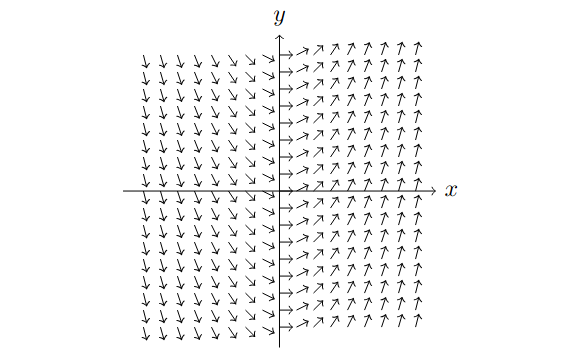
\includegraphics[width=10cm]{1}\\
\end{center}
(note that in this case $f(x,y)$ does not depend on $y$ (because of the equation)---it is invariant under vertical
translation)
\end{figure}\\
\textbf{Plotting direction fields---Isoclines}\\
In practice, computers are used to plot direction fields following the procedure:
\begin{enumerate}
\item Pick point $(x,y)$
\item Compute $y'=f(x,y)$
\item Plot line segment of slope at that point
\end{enumerate}
Notice how a new slope has to be computed for each specified point; when plotting direction fields by hand, 
it is much more practical to utilise \textit{isoclines}, which are, given the equation $y'=f(x,y)$, a one-parameter
family of curves given by the equations
\begin{equation*}
f(x,y)=m,\quad m\text{ constant}
\end{equation*}
Along a given isocline, all line segments have the same slope $m$.\\
(next page)
\newpage
\noindent\textbf{Example}\\
Consider plotting the direction field for the equation
$y'=x-y$; the isoclines are correspondingly the lines
$x-y=m$ (shown in dashed lines):
\begin{figure}[h]
\begin{center}
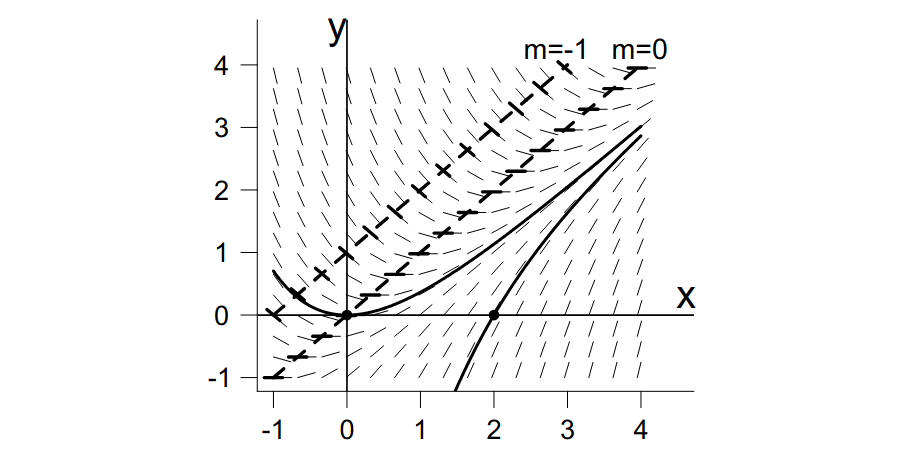
\includegraphics[width=10cm]{2}\\
\end{center}
The $m=0$ isocline marks the points where the slope of the solution is 0; it is therefore of special interest 
and is called the \textit{nullcline}.
\end{figure}\\
\textbf{Integral curves}\\
As also shown in the figure above, once the direction field has been sketched, curves which are \textit{at each
point tangent to the line segment at that point} can be drawn; 
such curves are called \textit{integral curves} or \textit{solution curves} for the direction field.
Their significance (this should be obvious) is that
\begin{equation*}
\text{\textit{The integral curves are the graphs of the solutions to }}y'=f(x,y)
\end{equation*}
Two integral curves have been drawn above (in solid lines).\\
\vspace{1mm}\\
\textbf{Intersection Principle}\\
Intuitively, see that at any point in the direction field it can only have one direction; therefore it is fairly
obvious that integral curves cannot cross at an angle.\\
\vspace{1mm}\\
Consider the existence and uniqueness theorem for ODEs: 
\begin{align*}
&\text{\textit{For any $(a,b)$ in the region where $f$ is defined, $y'=f(x,y)$ has}}\\&\text{\textit{exactly one solution such that 
$y(a)=b$.}}
\end{align*}
by the existence part of the theorem, 
there is an integral curve through any point where $f(x,y)$ is defined. Now supposing two integral curves
through the same point, by the uniqueness part of the theorem they must agree.\\
\vspace{1mm}\\
As a result, \textit{integral curves cannot intersect}; every point lies on exactly one integral curve.
\newpage

\subsection{Long term Behaviour: Fences, Funnels, and Separatrices}%140824
\textbf{Fences}\\
A \textit{lower fence} for the equation $y'=f(x,y)$ is a curve that `blocks' an integral curve from crossing from
\textit{above}; intuitively it is the curve whose direction field elements along the curve point up from it. Technically 
it can be described as a curve $y=L(x)$ such that $L'(x)<f(x,L(x))$ (the slope of the curve is always 
less than the slope of the direction field at that point).\\
\vspace{1mm}\\
Likewise an \textit{upper fence} is a curve that `blocks' integral curves from crossing from \textit{above}. 
Illustrated:
\begin{figure}[h]
\begin{center}
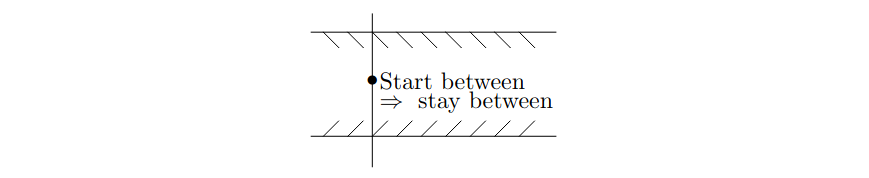
\includegraphics[width=10cm]{3}\\
\end{center}
(The upper curve is the upper fence and the lower curve is the lower fence). Solutions will be `squeezed' between
upper and lower fences.
\end{figure}\\
Note that
\begin{itemize}
\item Note that fences aren't necessarily defined for all $x$; they could be defined only on an interval like
$x\geq c$ for some constant $c$.
\item Since integral curves can't cross an integral curve itself it is both an upper and lower fence.
\end{itemize}
(next page)
\newpage
\noindent\textbf{Example}\\
Consider the direction field for the equation
\begin{equation*}
y'=y^2-x
\end{equation*}
The isoclines for $m=0$ and $m=-1$ are plotted in yellow, with integral curves in blue:
\begin{figure}[h]
\begin{center}
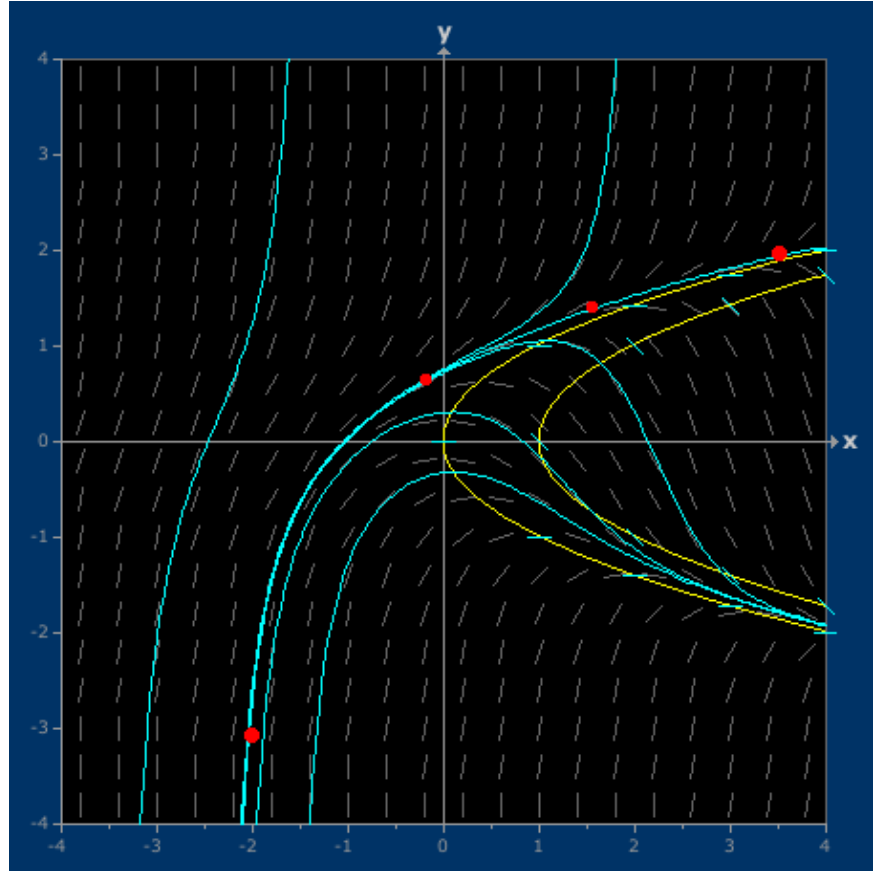
\includegraphics[width=10cm]{4}\\
\end{center}
Notice that the bottom hald of the isocline $m=0$ is a lower fence and for $x$ large enough the bottom 
half of the isocline $m=-1$ is an upper fence. (notice that the $m=-1$ isocline becomes an upper
fence only for $x$ large enough)
\end{figure}\\
(next page)
\newpage
\noindent\textbf{Funnels}\\
One use of fences is to construct funnels. A \textit{funnel} for the equation $y'=f(x,y)$ consists of a pair of 
fences; one lower fence $L(x)$ and one upper fence $U(x)$ with the properties
\begin{enumerate}
\item For $x$ large the lower fence is below the upper fence; $L(x)<U(x)$
\item The two fences come together asymptotically; $U(x)-L(x)$ is small for large $x$
\end{enumerate}
For instance, in the above example the bottom parts of the two isoclines $m=0$ and $m=-1$ act as a funnel
once $x$ is large enough. Given the equations of each isocline we have highly accurate estimates for solutions
between them as
\begin{equation*}
\underbrace{-\sqrt{x}}_{m=0}<y(x)<\underbrace{-\sqrt{x-1}}_{m=-1}
\end{equation*}
which is valid for large $x$.\\
\vspace{1mm}\\
Note that not all pairs of upper/lower fences form a funnel---they have to come together asymptotically as $x$ 
gets large.\\
\vspace{1mm}\\
\textbf{Separatrices}\\
A \textit{separatrix} is an integral curve such that the integral curves above it behave entirely differently from
integral curves below it as $x\to\infty$.
\newpage

\subsection{Runge-Kutta 2 (Numerical methods)}%161024
\textbf{General approach and Euler's method}\\
Euler's method (for numerical estimation) follows a more general procedure for stepping from 
$(x_n,y_n)$ to $(x_{n+1},y_{n+1})$:
\begin{equation*}
x_{n+1}=x_n+h,\quad y_{n+1}=y_n+m_nh
\end{equation*}
Where $h$ is the stepsize in the $x$ direction and $m$ is the slope of the line we step along. In Euler's
method $h$ is fixed ahead of time and $m_n=f(x_n,y_n)$.\\
\vspace{1mm}\\
\textbf{Runge-Kutta 2}\\
Naturally Euler's method is a fairly flawed method of numerical estimation. Other methods use other (and better)
ways of choosing $h$ and $m$. Here I describe the \textit{Runge-Kutta 2} (RK2) method, which is a
\textit{fixed stepsize} method; meaning $h$ is fixed and the added complexity comes from finding $m$.\\
\vspace{1mm}\\
Given an initial value problem $y'=f(x,y),y(x_0)=x_0$ and a step size $h$, one step of the RK2 method is as follows:
\begin{enumerate}
\item Compute the slope $k_1$ at $(x_0,y_0)$: $k_1=f(x_0,y_0)$
\item `Take' an Euler step from $(x_0,y_0)$ to $(a,b):$ $a=x_0+h,$  $b=y_0+k_1h$
\item Compute the slope $k_2$ at $(a,b):$ $k_2=f(a,b)$
\item Average $k_1$ and $k_2$ to get $m$: $m=(k_1+k_2)/2$
\item Now we use this averaged slope to take a step from 
$(x_n,y_n)$ to $(x_{n+1},y_{n+1})$: 
\begin{equation*}
x_{1}=x_0+h,\quad y_{1}=y_0+mh;\quad m=\frac{(k_1+k_2)}{2}
\end{equation*}
\end{enumerate}
Other methods such as RK4 or \textit{variable stepsize methods} may (probably) work better. Though one might want
to consider computational efficiency at the expense of accuracy.
\newpage

\subsection{First order Linear Differential Equations}%181024
\textbf{Definition}\\
The general \textit{First order linear ODE} in the unknown function $x=x(t)$ has the form
\begin{equation*}
A(t)\frac{dx}{dt}+B(t)x(t)=C(t)
\end{equation*}
If $A(t)\neq0$ we can simplify the equation by dividing by $A(t)$:
\begin{equation*}
\frac{dx}{dt}+p(t)x(t)=q(t)
\end{equation*}
This is called the \textit{standard form} for a first order linear ODE. Should the \textit{coefficients} $A(t),B(t)$
be constants (not dependent on $t$) we say the equation is a \textit{constant coefficient} DE.\\
\vspace{1mm}\\
If $C(t)=0$:
\begin{equation*}
A(t)\frac{dx}{dt}+B(t)x(t)=0
\end{equation*}
The DE is called \textit{homogeneous} (notice that conversion to standard form doesn't change this fact); otherwise
the equation is \textit{inhomogeneous}.\\
\vspace{1mm}\\
\textbf{Signals and Systems---Terminology}\\
Given a differential equation
\begin{equation*}
\frac{dx}{dt}+p(t)x(t)=q(t)
\end{equation*}
Notice that the right-hand side does not depend on $x$. The left-hand side represents the \textit{system}
(think of it as defining the behaviour of a system); the
right-hand side represents an outside influence on the system, which we can call the \textit{input}.\\
\vspace{1mm}\\
In general, a signal is a function of $t$. The system \textit{responds} to the input signal and yields
the function $x(t)$, which we call the \textit{output signal} or \textit{system response}. (these terms should just
be seen as convenient convention when describing an ODE)\\
\vspace{1mm}\\
\textit{Block diagrams} can be used to visually represent systems:
\begin{figure}[h]
\begin{center}
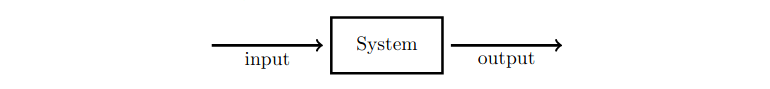
\includegraphics[width=10cm]{5}\\
\end{center}
(next page)
\end{figure}
\newpage
\noindent\textbf{Example---RC circuits}\\
Suppose we have an electrical circuit as shown
\begin{figure}[h]
\begin{center}
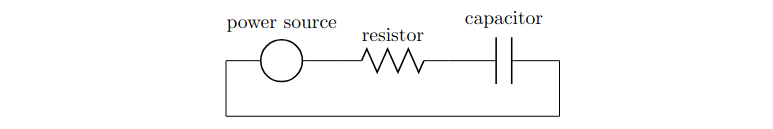
\includegraphics[width=10cm]{6}\\
\end{center}
``Kirchhoff's Voltage Law'' states that the total voltage change around the loop is 0, meaning
\begin{equation*}
V(t)=V_R(t)+V_C(t)
\end{equation*}
The relationship between voltage drop and current are described as follows:
\begin{align*}
&\text{Resistor: }V_R(t)=RI(t)\text{ for a constant }R,\text{ the ``resistance''}\\
&\text{Capacitor: }V'_C(t)=\frac{1}{C}I(t)\text{ for a constant }C,\text{ the ``capacitance''}
\end{align*}
the voltage drop from the capacitance can be seen from
the equation defining capacitance
\begin{align*}
q&=CV\quad\text{(charge per unit voltage)}\\
I(t)=\frac{dq}{dt}&=\frac{d}{dt}(CV)\\
I(t)&=CV'\quad\text{($C$ constant)}\\
V'_C(t)&=\frac{1}{C}I(t)
\end{align*}
The voltage drop across the capacitor is proportional to the \textit{integral} of the current; it results from
a buildup of charge on two plates of the capacitor.\\
(next page)
\end{figure}
\newpage
\noindent We can differentiate Kirchhoff's Voltage Law 
\begin{align*}
V'(t)&=V_R'(t)+V_C'(t)\\
&=RI'(t)+\frac{1}{C}I(t)
\end{align*}
to obtain a first order linear differential equation
\begin{equation*}
RI'(t)+\frac{1}{C}I(t)=V'(t)
\end{equation*}
In this circuit we consider the voltage $V(t)$ to be the input signal, and the circuit with resistance $R$ and
capacitance $C$ to be the system. The current $I$ is the output signal/system response:
\begin{figure}[h]
\begin{center}
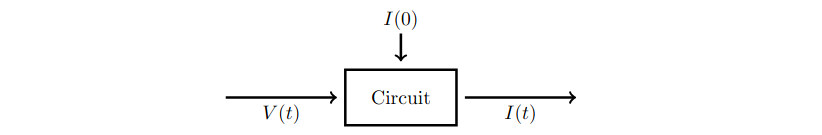
\includegraphics[width=10cm]{7}\\
\end{center}
$I(0)$ represents the initial condition.
\end{figure}
\newpage

\subsection{Superposition (First order ODEs)}%191024
Considering the following the first order linear equation:
\begin{equation*}
\dot{y}+p(t)y=q(t)
\end{equation*}
If a given input $q(t)$ has the output $y(t)$ we write
\begin{equation*}
q\rightsquigarrow y
\end{equation*}
Here we show that if
\begin{equation*}
q_1\rightsquigarrow y_1\text{ and }q_2\rightsquigarrow y_2
\quad\text{then}\quad c_1q_1+c_2q_2\rightsquigarrow
c_1y_1+c_2y_2
\end{equation*}
\textbf{Proof}\\
First see that (since differentiation does't change the constant coefficient)
\begin{align*}
\frac{dy}{dt}+py&=q\\
c\frac{dy}{dt}+cpy&=cq\\
=\frac{d(cy)}{dt}+p(cy)&=cq;\quad cq\rightsquigarrow cy
\end{align*}
Now see that
\begin{align*}
\frac{d(c_1y_1+c_2y_2)}{dt}+p(c_1y_1+c_2y_2)
&=\underbrace{c_1\dot{y}_1+pc_1y_1}_{=c_1q_1}
+\underbrace{c_2\dot{y}_2+pc_2y_2}_{=c_2q_2}\\
&=c_1q_1+c_2q_2
\end{align*}
Essentially, any linear combination of solutions is also a solution.
\newpage

\subsection{Solution by Integrating Factor (inhomogenous first order ODEs)}%240824
Here we prove the general solution to the inhomogeneous first order linear ODE 
\begin{equation*}
\dot{x}+p(t)x=q(t)
\end{equation*}
is\begin{equation*}
x(t)=\frac{1}{u(t)}\left(\int u(t)q(t)dt+C\right),
\quad\text{where }u(t)=e^{\int p(t)dt}
\end{equation*}
the function $u$ is called an \textit{integrating factor}.\\\vspace{1mm}\\
\textbf{Proof}\\
We start with the product rule for differentiation:
\begin{equation*}
\frac{d}{dt}(ux)=u\dot{x}+\dot{u}x
\end{equation*}
Consider multiplying both sides of our inhomogenous first order ODE by some function $u(t)$:
\begin{equation*}
u\dot{x}+upx=uq
\end{equation*}
We want to choose a function $u(t)$ such that we can apply the product rule to the sum on the left hand side
of the equation. There may be many functions $u$ that could work, but in this case we only need one. See that
\begin{equation*}
\frac{d}{dt}(ux)=u\dot{x}+\dot{u}x\iff u\dot{x}+upx=u\dot{x}+\dot{u}x\iff
\dot{u}=up
\end{equation*}
so now by separation of equations
\begin{align*}
\frac{du}{u}&=p(t)dt\\
\ln|u|&=\int p(t)dt\\
u&=e^{\int p\,dt}
\end{align*}
By using $u$ to satisfy the product rule:
\begin{align*}
u\dot{x}+upx=\frac{d}{dt}(ux)&=uq\\
u(t)x(t)&=\int u(t)q(t)dt+c\\
x(t)&=\frac{1}{u(t)}\left(\int u(t)q(t)dt+c\right)
\end{align*}
which was what we wanted.\\
(next page)
\newpage
\noindent\textbf{Integrating factor and homogeneous equations}\\
Given the homogeneous first order ODE
\begin{equation*}
\dot{x}+p(t)x=0
\end{equation*}
Solving by separation of variables gives
\begin{equation*}
x_h(t)=Ae^{-\int p(t)dt}
\end{equation*}
Comparing this to the formula for the integrating factor
\begin{equation*}
u(t)=e^{\int p(t)dt}
\end{equation*}
see that
\begin{equation*}
x_h(t)=\frac{A}{u(t)}
\end{equation*}
\newpage

\subsection{General, Particular and Homogeneous solutions}%301024
Solving by method of Integrating factors allows us to come up with a solution for inhomogeneous first order linear
ODEs
\begin{equation*}
\dot{x}+p(t)x=q(t)
\end{equation*}
Which have the form
\begin{equation*}
x(t)=\frac{1}{u(t)}\left(\int u(t)q(t)dt+C\right),
\quad\text{where }u(t)=e^{\int p(t)dt}
\end{equation*}
Notice that the presence of the constant $C$ implies a family of solutions; by setting $C=0$ we get a
\textit{particular solution} $x_p$, which is simply one specific solution---we could have chosen any other:
\begin{align*}
x_p=\frac{1}{u(t)}\left(\int u(t)q(t)dt+0\right)\quad&\text{is a solution}\\
x_p=\frac{1}{u(t)}\left(\int u(t)q(t)dt+999\right)\quad&\text{is also a solution}
\end{align*}
The method of integrating factors naturally leaves us with a constant. But say we were to find a solution by 
\textit{inspection}---how would we know that the constant of integration exists in the form $\frac{C}{u(t)}$? (as
is in this case)\\
\vspace{1mm}\\
\textbf{General solution}\\
See that since
\begin{equation*}
x_h(t)=\frac{1}{u(t)}
\end{equation*}
We can write the solution by integrating factor as
\begin{align*}
x(t)&=\frac{1}{u(t)}\left(\int u(t)q(t)dt\right)+\frac{C}{u(t)}\\
&=x_p+Cx_h
\end{align*}
One way to fully solve the inhomogeneous equation is by first solving the \textit{homogeneous} equation, and
then finding any \textit{one} solution, a \textit{particular solution}, to the inhomogeneous equation $x_p$. 
(We can use any method to find $x_p$ since we the homogeneous solution handles the constant of integration):
\begin{equation*}
\text{General solution}=\text{Particular solution}+\text{Homogeneous solution}
\end{equation*}
(next page)
\newpage
\noindent\textbf{Intuition}\\
Given an inhomogeneous first order linear ODE and its associated homogeneous equation
\begin{align*}
\dot{x}+p(t)x=q(t)\quad&\text{(inhomogeneous)}\\
\dot{x}+p(t)x=0\quad&\text{(homogeneous)}
\end{align*}
Solving both equations by method of integrating factors gives
\begin{equation*}
x_p(t)=\frac{1}{u(t)}\left(\int u(t)q(t)dt\right)+\frac{A}{u(t)},\qquad
x_h(t)=\frac{B}{u(t)}
\end{equation*}
(where $A$ is any chosen constant, each constant giving a particular solution, and $B$ the constant of integration)
Now see that by adding the solutions together the constant for the inhomogeneous solution $A$ gets absorbed into
the homogeneous solution:
\begin{align*}
x_p(t)+x_h(t)&=\frac{1}{u(t)}\left(\int u(t)q(t)dt\right)+\frac{A+B}{u(t)}\\
&=\frac{1}{u(t)}\left(\int u(t)q(t)dt\right)+\frac{C}{u(t)}
\end{align*}
We can obtain the `ambiguous part' of the general solution by simply solving the homogeneous equation; this means
that when obtaining a particular solution we don't have to worry about the constant of integration.\\
\vspace{1mm}\\
\textbf{Superposition}\\
See that this also makes sense with respect to superposition of solutions, where since
\begin{equation*}
\underbrace{q(t)\rightsquigarrow x_p(t)}_{\text{inhomogeneous}}\quad\text{and}\quad
\underbrace{0\rightsquigarrow x_h(t)}_{\text{homogeneous}}
\end{equation*}
we can say
\begin{equation*}
q(t)+0=q(t)\rightsquigarrow x_p(t)+x_h(t)
\end{equation*}
\newpage

\subsection{Polar form and Euler Identity}%311024
\textbf{The Complex Plane, Polar Form}\\
Complex numbers can be represented geometrically by points in a plane, where the number $a+ib$ is represented by 
the point $(a,b)$; when points in a plane are thought of as representing complex numbers this way,
the plane is known as a \textit{Complex Plane}:
\begin{figure}[h]
\begin{center}
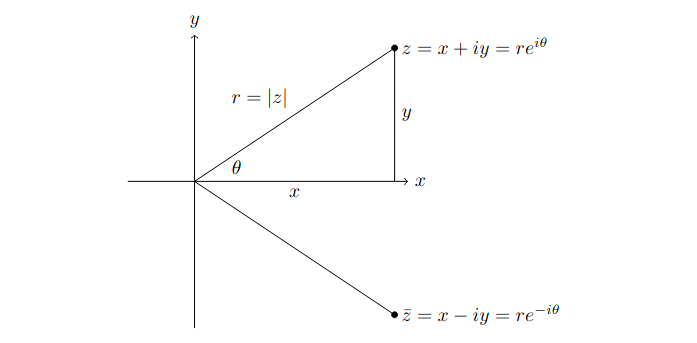
\includegraphics[width=9cm]{8}\\
\end{center}
See that the magnitude of the coordinates of a complex number $x+iy$ can be represented by
\begin{equation*}
x=r\cos(\theta),\quad y=r\sin(\theta)
\end{equation*}
where $r$ is the absolute value of the number:
\begin{equation*}
r=|x+iy|=\sqrt{x^2+y^2}
\end{equation*}
(its just the pythagorean theorem) thus the entire number
can be written as
\begin{equation*}
x+iy=r(\cos(\theta)+i\sin(\theta))
\end{equation*}
This is called the \textit{Polar Form}
of a non-zero complex number. We call $\theta$ the \textit{angle} or
\textit{argument} of $x+iy$:
\begin{equation*}
\theta=\arg(x+iy)
\end{equation*}
Notice that the angle can be increased by any integer multiple of $2\pi$ and will still represent the same thing. 
To simplify this one can specify the \textit{principal value} of the angle:
\begin{equation*}
0\leq\theta<2\pi
\end{equation*}
this can be indicated by $\text{Arg}(...)$; for instance
\begin{equation*}
\text{Arg}(-1)=\pi,\quad\arg(-1)=\pm\pi,\pm3\pi,\pm5\pi
\end{equation*}
\end{figure}\\
(next page)
\newpage
\noindent\textbf{Euler's Formula}\\
Complex numbers have another \textit{exponential} form called \textit{Euler's formula}:
\begin{equation*}
e^{i\theta}=\cos(\theta)+i\sin(\theta)
\end{equation*}
This should be regarded as a definition for the exponential of an imaginary power.\\
\vspace{1mm}\\
A good justification for Euler's formula can be found from
its Taylor approximation:
\begin{align*}
e^{i\theta}&=1+i\theta-\frac{\theta^2}{2!}-i\frac{\theta^3}{3!}+\frac{\theta^4}{4!}+i\frac{\theta^5}{5!}-\cdots\\
&=\left(1-\frac{\theta^2}{2!}+\frac{\theta^4}{4!}-\cdots\right)+i\left(\theta-\frac{\theta^3}{3!}
+\frac{\theta^5}{5!}-\cdots\right)\\
&=\cos(\theta)+i\sin(\theta)
\end{align*}
Note that the argument above is not a proof; rather it just shows that Euler's formula is formally compatible with
the series expansions for the exponential, sine, and cosine functions.\\
\vspace{1mm}\\
\textbf{Polar form again}\\
We can now write
\begin{equation*}
x+iy=r(\cos(\theta)+i\sin(\theta))=re^{i\theta}
\end{equation*}
Polar representation in exponential form allows for much simpler multiplication of complex numbers. Since one can
show that (using angle addition formulas)
\begin{align*}
e^{i\theta_1}e^{i\theta_2}&=(\cos(\theta_1)+i\sin(\theta_1))(\cos(\theta_2)+i\sin(\theta_2))\\
&=\cos(\theta_1)\cos(\theta_2)-\sin(\theta_1)\sin(\theta_2)\\&\quad+i(\sin(\theta_1)\cos(\theta_2)+\cos(\theta_1)\sin(\theta_2)\\
&=\cos(\theta_1+\theta_2)+i\sin(\theta_1+\theta_2)\\
&=e^{i(\theta_1+\theta_2)}
\end{align*}
(next page)
\newpage
\noindent\textbf{Complex Exponential properties}\\
We had
\begin{equation*}
e^{i\theta_1}e^{i\theta_2}=e^{i(\theta_1+\theta_2)}
\end{equation*}
This property can be extrapolated to further justify Euler's formula---the complex exponential follows
the same exponential addition rules as any typical exponential. See that we can now conclude:\\
\vspace{1mm}\\
\textit{Multiplication rule:}
\begin{equation*}
r_1e^{i\theta_1}\cdot r_2e^{i\theta_2}=r_1r_2e^{i(\theta_1+\theta_2)}
\end{equation*}
also see that since
\begin{equation*}
\frac{1}{r}e^{-i\theta}\cdot re^{i\theta}=1
\end{equation*}
\textit{Reciprocal Rule:} 
\begin{equation*}
\frac{1}{re^{i\theta}}=\frac{1}{r}e^{-i\theta}
\end{equation*}
\textbf{DeMoivre's Formula}\\
Since 
\begin{equation*}
(x+iy)^n=r^ne^{in\theta}
\end{equation*}
we can show \textit{DeMoivre's formula:}
\begin{equation*}
(\cos(\theta)+i\sin(\theta))^n=e^{in\theta}=\cos(n\theta)+i\sin(n\theta)
\end{equation*}
\textbf{Combining pure oscillations of the same frequency}\\
We can also show that
\begin{equation*}
a\cos(\lambda t)+b\sin(\lambda t)=A\cos(\lambda t-\phi)
\end{equation*}
where
\begin{equation*}
A=\sqrt{a^2+b^2},\quad\phi=\tan^{-1}\left(\frac{b}{a}\right)
\end{equation*}
See that
\begin{align*}
a\cos(\lambda t)+b\sin(\lambda t)&=\text{Re}((a-bi)(\cos(\lambda t)+i\sin(\lambda t))\\
&=\text{Re}(Ae^{-i\phi}\cdot e^{i\lambda t})\\
&=\text{Re}(Ae^{i(\lambda t-\phi)})\\
&=A\cos(\lambda t-\phi)
\end{align*}
\newpage

\subsection{More on Complex Exponentials}%031124
\textbf{Notable properties}\\
We know that (as proven)
\begin{equation*}
e^{a+ib}=e^ae^{ib}=e^a(\cos(b)+i\sin(b))
\end{equation*}
So see that
\begin{equation*}
\text{Re}(e^{a+ib})=e^a\cos(b),\quad
\text{Im}(e^{a+ib})=e^a\sin(b)
\end{equation*}
this can be extrapolated further to show
\begin{align*}
\cos(x)&=\text{Re}(e^{ix}),&\sin(x)&=\text{Im}(e^{ix})\\
\cos(x)&=\frac{1}{2}(e^{ix}+e^{-ix}),&\sin(x)&=
\frac{1}{2i}(e^{ix}-e^{-ix})
\end{align*}
\textbf{Derivatives and integrals}\\
Note that a function like
\begin{equation*}
e^{ix}=\cos(x)+i\sin(x)
\end{equation*}
is a \textit{complex-valued function of the real variable} $x$. Such a function may be written as
\begin{equation*}
u(x)+iv(x),\quad u,v\text{ real-valued}
\end{equation*}
with its derivative and integral with respect to $x$ defined to be
\begin{equation*}
\text{a) }D(u+iv)=Du+iDv,\quad\text{b) }\int(u+iv)dx=\int udx+i\int vdx
\end{equation*}
It follows easily that
\begin{equation*}
D(e^{(a+ib)x})=(a+ib)e^{(a+ib)x}
\end{equation*}
since
\begin{align*}
D(e^{(a+ib)x})&=D(e^{ax}\cos(bx)+ie^{ax}\sin(bx))\\
&=ae^{ax}\cos(bx)-be^{ax}\sin(bx)+i(ae^{ax}\sin(bx)+be^{ax}\cos(bx))\\
&=e^{ax}\cos(bx)(a+ib)+e^{ax}\sin(bx)(ia+i^2b)\\
&=(a+ib)e^{ax}(\cos(bx)+i\sin(bx))\\
&=(a+ib)e^{(a+ib)x}
\end{align*}
Therefore we can also write the down the integral as
\begin{equation*}
\int e^{(a+ib)x}dx=\frac{1}{a+ib}e^{(a+ib)x}
\end{equation*}
\newpage

\subsection{Finding $n$-th roots}
To solve linear DEs with constant coefficients, we need to be able to find the real and complex roots of polynomial
equations. Though a lot of this is done today with calculators and computers, one
still has to know how to do an important special case by hand: finding the roots of 
\begin{equation*}
z^n=\alpha
\end{equation*}
where $\alpha$ is a complex number---finding the $n$-th roots of $\alpha$.\\
\vspace{1mm}\\
\textbf{$n$-th roots of unity}\\
Consider first a special case; we want the solutions to
\begin{equation*}
z^n=1
\end{equation*}
We use polar representation for both sides, setting $z=re^{i\theta}$ on the left. See that
\begin{equation*}
\underbrace{r^ne^{in\theta}}_{(re^{i\theta})^n}
=\underbrace{1\cdot e^{(2k\pi i)},\quad k=0,\pm1,\pm2,\ldots}_{=1}
\end{equation*}
Equating the absolute values and the arguments of each side:
\begin{equation*}
r^n=1,\quad n\theta=2k\pi,\quad k=0,\pm1,\pm2,\ldots
\end{equation*}
(Notice the arguments for $k=a$ and $k=-a$, where $a$ is an integer, are the same.
Also see that $r$ can only be 1 it is defined to be \textit{real and non-negative} 
so it can't be anything else) we can conclude that
\begin{equation*}
r=1,\quad\theta=\frac{2k\pi}{n},\quad k=0,1,\ldots,n-1
\end{equation*}
we don't need any integer values of $k$ other than $0,\ldots,n-1$---they would not produce a complex number
that isn't already among the above $n$ numbers. See that if we add $an$, an integer multiple of $n$,
to any $k$ we get the same complex number:
\begin{equation*}
\theta'=\frac{2(k+an)\pi}{n}=\theta+2a\pi\end{equation*}
(this is the same as having $k=n,n+1,n+2\ldots$) so
\begin{equation*}
e^{i\theta'}=e^{i\theta}e^{2a\pi i}=e^{i\theta}
\end{equation*}
We can conclude therefore that \textit{the $n$-th roots of 1 are the numbers}
\begin{equation*}
e^{2k\pi i/n},\quad k=0,\ldots,n-1
\end{equation*}
(next page)
\newpage
\noindent\textbf{Roots of unity visualised}\\
There are $n$ complex $n$-th roots of unity. Since they all have absolute value 1 ($r=1$) they all lie on the unit
circle in the complex plane. They are evenly spaced around the unit circle; the angle between two consecuitive
roots is $2\pi/n$.
\begin{figure}[h]
Illustrated here is the case for $n=6$:
\begin{center}
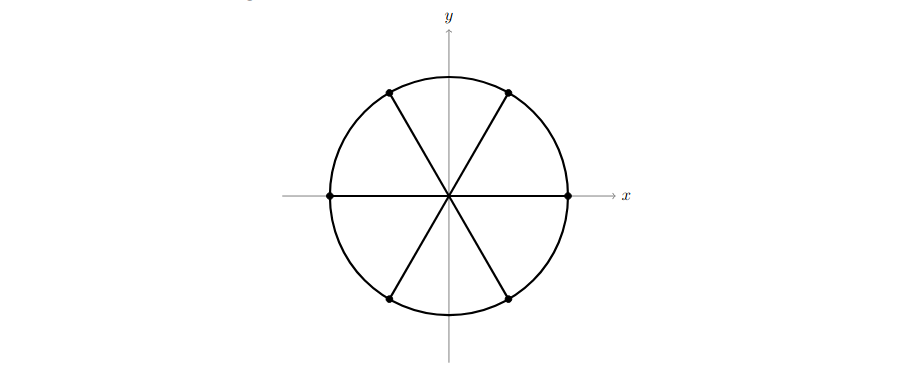
\includegraphics[width=10cm]{9}\\
\end{center}
The six solutions to $z^6=1$ lie on the unit circle in the complex plane. 
See that we can express the roots of unity in
a different notation:
\begin{equation*}
\text{\textit{the $n$-th roots of 1 are} }1,\zeta,\zeta^2,\ldots,\zeta^{n-1},\text{ where }\zeta=e^{2\pi i/n}
\end{equation*}
\end{figure}\\
\textbf{General case}\\
Now we generalise to find the $n$-th roots of an arbitrary complex number $w$. We start by writing $w$ in
polar form:
\begin{equation*}
w=re^{i\theta};\quad\theta=\text{Arg}(w),0\leq\theta<2\pi
\end{equation*}
Here $\theta$ is the principal value of the polar angle of $w$. Following the same reasoning as before, see that
\begin{equation*}
z^n=re^{i(\theta+2\pi k)};\quad k=0,\pm1,\pm2,\ldots
\end{equation*}
where removing the redundant $k$  (this can be shown using the same methods as above) and solving gives us
\begin{equation*}
z=\sqrt[n]{r}e^{i(\theta+2\pi k)/n},\quad k=0,1,\ldots,n-1
\end{equation*}
See that these $n$ roots can be expressed with the roots of unity as
\begin{equation*}
\sqrt[n]{w}=z_0,z_0\zeta,z_0\zeta^2,\ldots,z_0\zeta^{n-1},\quad\text{where }z_0=\sqrt[n]{r}e^{i\theta/n}
\end{equation*}
($z_0$ is just the case where $k=0$) See that all of the $n$ roots satisfy $z^n=w$.
\newpage

\subsection{Sinusoidal functions}
\textbf{Definition and properties}\\
A \textit{sinusoidal function/oscillation/signal} is one
that can be written in the from
\begin{equation*}
f(t)=A\cos(\omega t-\phi)
\end{equation*}
The function $f(t)$ is a cosine function which has been 
\textit{amplified} by $A$, \textit{shifted} by $\phi/\omega$, and \textit{compressed} by $\omega$.
\begin{itemize}
\item$A>0$ is its \textit{amplitude}: how high the graph of $f(t)$ rises above the $t$-axis at its maximum values
\item$\phi$ is its \textit{phase lag}: the value of $\omega t$ for which the graph has its maximum 
(a positive phase lag shifts the sinusoid \textit{forward}; consider a maximum at $\cos(a)$, 
without phase lag it is reached at $\omega t=a$, with phase lag its now $\omega t=a+\phi$.)
\item$\tau=\phi/\omega$ is its \textit{time delay/lag}: how far along the $t$-axis the graph of $\cos(wt)$ has been 
shifted due to phase lag. ($\tau$ and $\phi$ have the same sign; consider a maximum at $\cos(0)$, without
phase lag it is reached at $\omega t=0\implies t=0$, with phase lag its now 
$\omega t-\phi=0\implies t=\phi/\omega$.)
\item$\omega$ is its \textit{angular frequency}: the number of complete oscillations $f(t)$ makes per time interval
of $2\pi$; that is, the \textit{number of radians per unit time} 
(1 radian in 1 second means 1 oscillation in $2\pi$ seconds---1 radian is the angle subtended at the centre of 
a circle by an arc equal in length to the radius).
\item$v=\omega/2\pi$ is the \textit{frequency} of $f(t)$: the number of complete oscillations made in a
time interval of 1; that is, the number of cycles per unit time.
\item$P=2\pi/\omega=1/v$ is its \textit{period}: the $t$-interval required for one complete oscillation.
\end{itemize}
See that one can also write the sinusoidal function using
the time lag $\tau=\phi/\omega$:
\begin{equation*}
f(t)=A\cos(\omega(t-\tau))
\end{equation*}
(next page)
\newpage
\noindent\textbf{Example}\\
\begin{figure}[h]
In the figure below the dotted curve is $\cos(t)$ and the solid curve is $2.5\cos(\pi t-\pi/2)$. The solid
curve has
\begin{equation*}
A=2.5,\quad\omega=\pi,\quad\phi=\pi/2,\quad\tau=1/2
\end{equation*}
\begin{center}
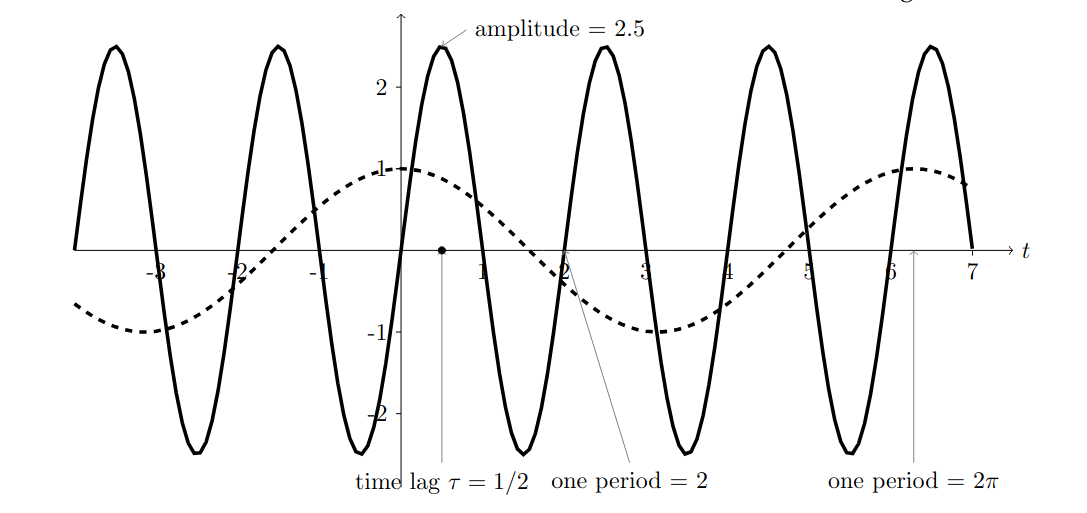
\includegraphics[width=10cm]{10}\\
\end{center}
\end{figure}
\newpage

\subsection{Solution to the Constant Coefficient First Order Equation}
\textbf{Solution}\\
Considering the constant coefficient equation (constant coefficient meaning $k$ is a constant)
\begin{equation*}
\dot{y}+ky=q(t)
\end{equation*}
This is easily solvable by integrating factor:
\begin{align*}
y&=e^{-kt}\left(\int e^{kt}q(t)dt+c\right)\\
&=e^{-kt}\int e^{kt}q(t)dt+ce^{-kt}
\end{align*}
(integrating factor gives us a way of finding the particular solution, but see that it also gives us the 
homogeneous solution) We have the \textit{particular} solution and \textit{homogeneous} solution respectively
\begin{equation*}
y_p(t)=e^{-kt}\int e^{kt}q(t)dt\quad\text{and}\quad
y_h(t)=e^{-kt}
\end{equation*}
The general solution is then
\begin{equation*}
y(t)=y_p(t)+cy_h(t)
\end{equation*}
\textbf{Behaviour for $k>0$:}\\
For $k>0$ the system models \textit{exponential decay}. When the input is 0 the system response is $y(t)=ce^{-kt}$, 
which decays exponentially to 0 as $t$ goes to $\infty$.\\
\vspace{1mm}\\
In the general solution we call $ce^{-kt}$ the \textit{transient} because it goes to 0. The other term 
$e^{-kt}\int e^{kt}q(t)dt$ is called the \textit{steady-state/long-term} solution. That is, $cy_h$ is the transient
and $y_p$ is the steady-state solution.\\
\vspace{1mm}\\
The value of $c$ is determined by the initial value $y(0)$. See that this initial value only affects the transient
and not the long-term behaviour of the solution---no matter what the initial condition, every solution goes
asymptotically to the steady-state---all solution curves approach the steady-state as $t\to\infty$.\\
\vspace{1mm}\\
(next page)
\newpage
\noindent\textbf{Behaviour for $k>0$ illustrated}\\
In the case $k>0$ all solutions go asymptotically to the 
steady-state:
\begin{figure}[h]
\begin{center}
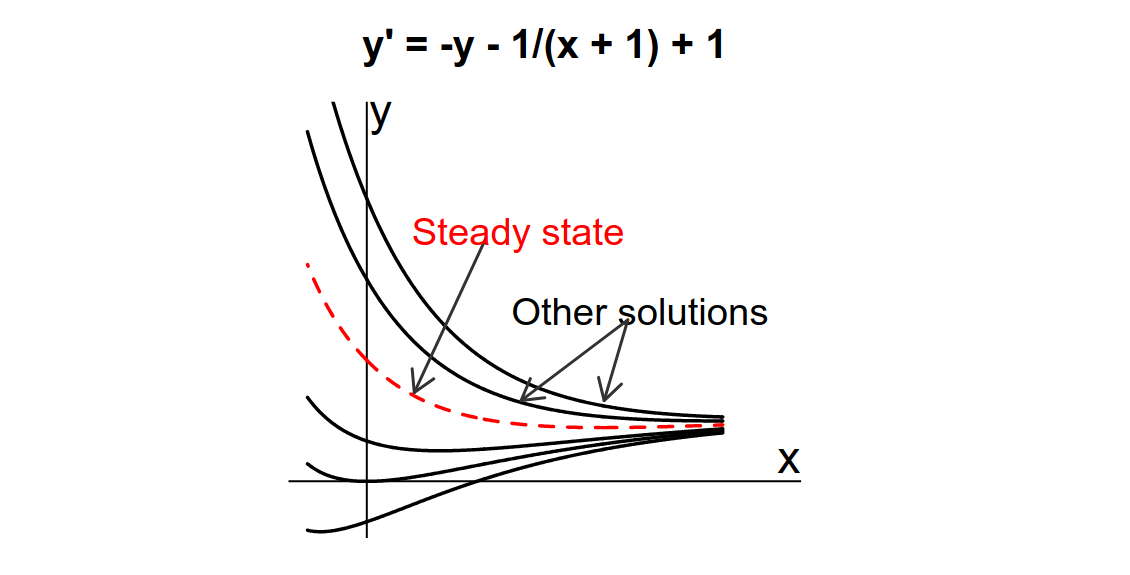
\includegraphics[width=10cm]{11}\\
\end{center}
Since all the solutions approach each other, there is no precise way to choose the one to we call the 
steady-state---we can \textit{choose any one} to be the steady-state solution. 
Generally we just choose the simplest looking solution.
\end{figure}\\
\textbf{The case $k\leq0$:}\\
When $k\leq0$ the homogeneous solution $e^-{kt}$ does not decay asymptotically to 0---it is not transient. In this
case it does not make sense to talk about the steady-state solution.
\newpage

\subsection{First Order Response to Sinusoidal/Exponential Input---complex replacement}
\textbf{Context}\\
Consider solving the first order constant coefficient DE with sinusoidal input
\begin{equation*}
\dot{x}+kx=B\cos(\omega t)
\end{equation*}
The idea here is to replace $\cos(\omega t)$ by the complex exponenial $e^{i\omega t}$; this is called
\textit{complex replacement}.\\
\vspace{1mm}\\
\textbf{Complex Replacement}\\
Consider introducing a new variable $y$ with its own related ODE:
\begin{equation*}
\dot{y}+ky=B\sin(\omega t)
\end{equation*}
Combining $x$ and $y$ to make a complex variable $z=x+iy$, see that we get
\begin{equation*}
\dot{z}+kz=B(\cos(\omega t)+i\sin(\omega t))=Be^{i\omega t}
\end{equation*}
where
\begin{equation*}
\cos(\omega t)=\text{Re}(e^{i\omega t})\quad\text{and}\quad x=\text{Re}(z)
\end{equation*}
\textbf{Exponential input}\\
Using complex replacement we now have the same problem but with exponential input
\begin{equation*}
\dot{z}+kz=Be^{i\omega t}
\end{equation*}
This can be solved using integrating factors, but we present a simpler solution: consider a particular solution of 
the form $z_p(t)=Ae^{i\omega t}$ (this is a reasonable choice given that differentiation reproduces exponentials); 
this gives us
\begin{equation*}
\dot{z}_p+kz_p=i\omega Ae^{i\omega t}+kAe^{i\omega t}
=(k+i\omega)Ae^{i\omega t}
\end{equation*}
so we have
\begin{equation*}
(k+i\omega)Ae^{i\omega t}=Be^{i\omega t}\implies A=B/(k+i\omega)
\end{equation*}
As such we have the particular solution
\begin{equation*}
z_p(t)=Be^{i\omega t}/(k+i\omega)
\end{equation*}
simplifying with polar coordinates:
\begin{equation*}
z_p(t)=\frac{Be^{i\omega t}}{\sqrt{k^2+\omega^2}e^{i\phi}}
=\frac{Be^{i(\omega t-\phi)}}{\sqrt{k^2+\omega^2}}
\end{equation*}
since
\begin{equation*}
k+i\omega=\sqrt{k^2+\omega^2}e^{i\phi},\quad\text{where }\phi=\tan^{-1}(\omega/k)\text{ in the first quadrant}
\end{equation*}
Since $\tan^{-1}$ is ambiguous ($\tan(\pi/4)=\tan(5\pi/4)=1$), we clarify by saying which quadrant the
complex number is in. In this case since $k,\omega>0$ its the first quadrant.\\
(next page)
\newpage
\noindent\textbf{Solving for sinusoidal input}\\
We have 
\begin{equation*}
z_p(t)=\frac{Be^{i(\omega t-\phi)}}{\sqrt{k^2+\omega^2}}
\end{equation*}
we wanted $x_p$, where $x_p=\text{Re}(z_p)$:
\begin{equation*}
x_p(t)=\frac{B}{\sqrt{k^2+\omega^2}}\cos(\omega t-\phi)
\end{equation*}
To get the general solution we add the homogeneous solution:
\begin{equation*}
x(t)=x_p(t)+Ce^{-kt}=\frac{B}{\sqrt{k^2+\omega^2}}\cos(\omega t-\phi)+Ce^{-kt}
\end{equation*}
\newpage

\subsection{Amplitude, Phase, Gain, and Bode Plots\\---Terminology and introduction}
\textbf{Terminology}\\
We found that the ODE
\begin{equation*}
\dot{x}+kx=kB\cos(\omega t)
\end{equation*}
has a particular solution
\begin{equation*}
x(t)=\frac{kB}{\sqrt{k^2+\omega^2}}\cos(\omega t-\phi)
\end{equation*}
where $\phi=\tan^{-1}(\omega/k)$. If we consider the input to be $B\cos(\omega t)$ then the 
gain $g$ (output amplitude/input amplitude) is $g=k/\sqrt{k^2+\omega^2}$:
\begin{equation*}
x(t)=gB\cos(\omega t-\phi)
\end{equation*}
We define the terminology as follows:
\begin{itemize}
\item $B\cos(\omega t)$ is the input/input signal.
\item $B$ is the input amplitude and $\omega$ is the input angular/circular frequency.
\item $x(t)$ is the output or response.
\item $g=k/\sqrt{k^2+\omega^2}$ is called the gain/amplitude response. 
See that the input amplitude is scaled by the gain to give the output amplitude.
\item $\phi$ is called the phase lag.
\end{itemize}
(next page)
\newpage
\noindent\textbf{Bode plots}\\
Since $g$ and $\phi$ vary with 
$\omega$, we can regard them as functions of $\omega$---$g(\omega)$ and $\phi(\omega)$.
$k$ is called the \textit{coupling constant}. Consider the graphs of $g(\omega)$ and $-\phi(\omega)$ for 
the values of coupling constant $k=.25,.5,.75,1,1.25,1.5$:
\begin{figure}[h]
\begin{center}
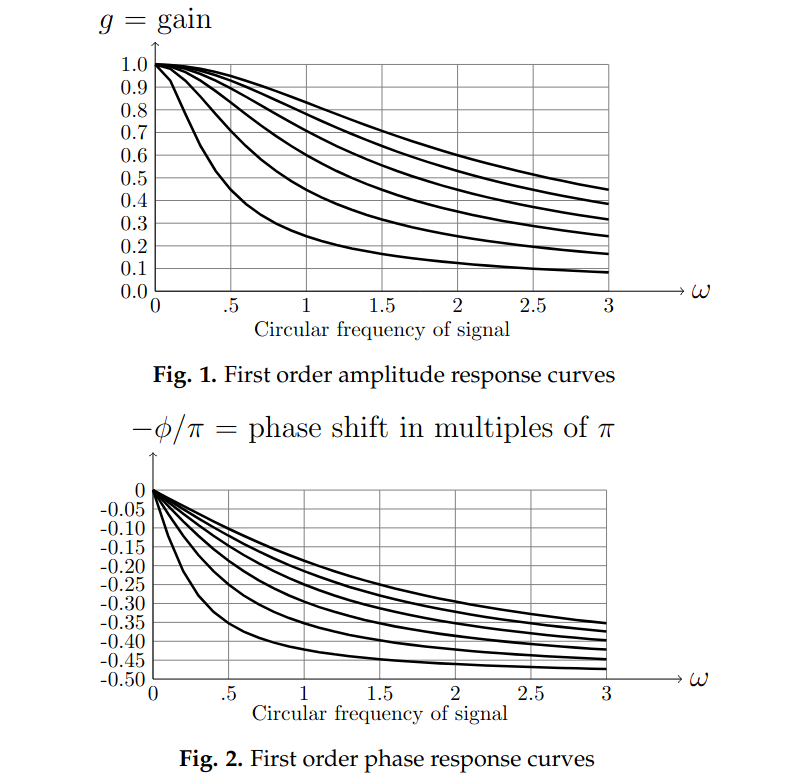
\includegraphics[width=10cm]{12}\\
\end{center}
\end{figure}\\
These graphs are essentially \textit{Bode plots}. (Bode plots display $\log g(\omega)$ and $-\phi(\omega)$ against 
$\log\omega$).
\newpage

\subsection{Autonomous equations, Logistic Model,\\Stable/Unstable equilibria}
Here we consider \textit{autonomous first order differential equations}. These are (in general) nonlinear equations
of the form
\begin{equation*}
\dot{x}=f(x)
\end{equation*}
(compare this with the general first order ODE $\dot{x}=f(x,t)$.) The word autonomous means self governing---the
rate of change of $x$ is governed by $x$ itself and is not dependent on time.\\
\vspace{1mm}\\
\textbf{Example: Logistic Population Model}\\
Suppose we have a model for a population $y$ with variable growth rate $k(y)$ which depends on the current
population but \textit{not on time}:
\begin{equation*}
\dot{y}=k(y)\cdot y
\end{equation*}
Say we model $k(y)$ as
\begin{figure}[h]
\begin{equation*}
k(y)=k_0\left(1-\frac{y}{M}\right)
\end{equation*}
\begin{center}
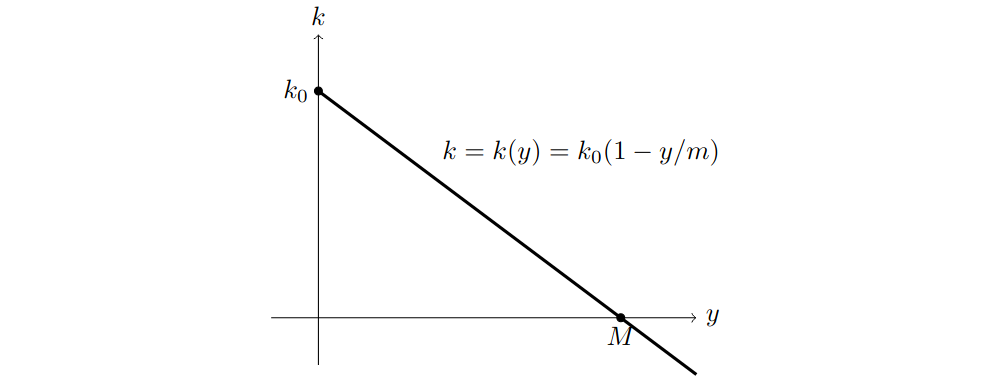
\includegraphics[width=10cm]{13}\\
\end{center}
\end{figure}\\
The idea here is that population growth is positive until the population reaches some $M$, after which it becomes 
negative and declines until it becomes lower than $M$.
In the simplest version of this we model $k(y)$ as a straight line as above. The final equation is known as the 
\textit{logistic population model}:
\begin{equation*}
\dot{y}=k_0(1-(y/M))y=f(y)
\end{equation*}
The equation is nonlinear and autonomous. 
Autonomous equations are always separable; in this case partial fractions could be used to compute an
integral, but here we consider a qualitative approach.\\
(next page)
\newpage
\noindent\textbf{Qualitative perspective}\\
We start by looking for \textit{constant} solutions
$y(t)=y_0$. We do this by considering $\dot{y}=0$; see that this occurs in two situations, either
\begin{equation*}
y(t)=0,\quad\text{or}\quad y(t)=M
\end{equation*}
Because a system at equilibrium is unchanging, we call these solutions \textit{equilibrium solutions}. 
Since equilibrium is achieved when $y$ is $0$ or $M$ we call $0$ and $M$ the \textit{critical points} of the DE. 
To summarise, these statements all mean the same thing:
\begin{enumerate}
\item $f(y_0)=0$.
\item $y(t)=y_0$ is an equilibrium solution.
\item $y=y_0$ is a critical point.
\end{enumerate}
Consider the direction field for these solutions; (recall each isocline represents $f(y)=c$) they correspond to the
\textit{nullclines}, where $f(y)=0$:
\begin{figure}[h]
\begin{center}
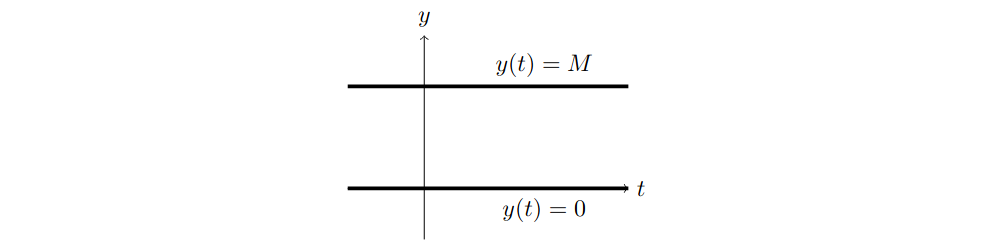
\includegraphics[width=10cm]{14}\\
\end{center}
\end{figure}\\
(Note that the nullclines are also solution curves, if $y$ starts at $M$ it will never change since its
derivative will be 0 forever.) For a clear picture of the other isoclines consider
a graph of $f(y)$ against $y$:
\begin{figure}[h]
\begin{center}
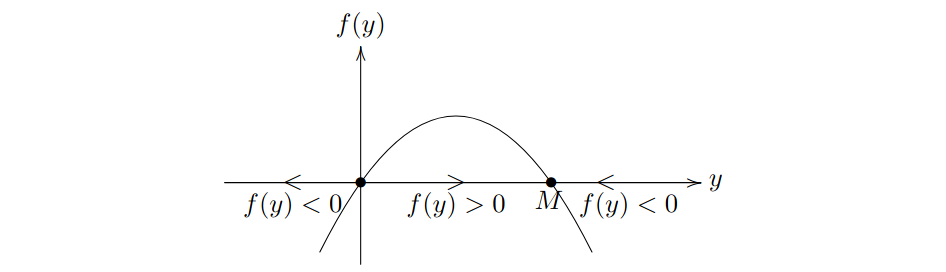
\includegraphics[width=10cm]{15}\\
\end{center}
\end{figure}\\
See that 
\begin{align*}
\text{for }y<0\quad&\dot{y}=f(y)\text{ is negative,}\\
\text{for }0<y<M\quad&\dot{y}=f(y)\text{ is positive,}\\
\text{for }M<y\quad&\dot{y}=f(y)\text{ is negative}
\end{align*}
These are indicated on the graph by the arrows on the horizontal axis.\\
(next page)
\newpage
\noindent\textbf{Direction field}\\
We sketch the direction field and some solution curves:
\begin{figure}[h]
\begin{center}
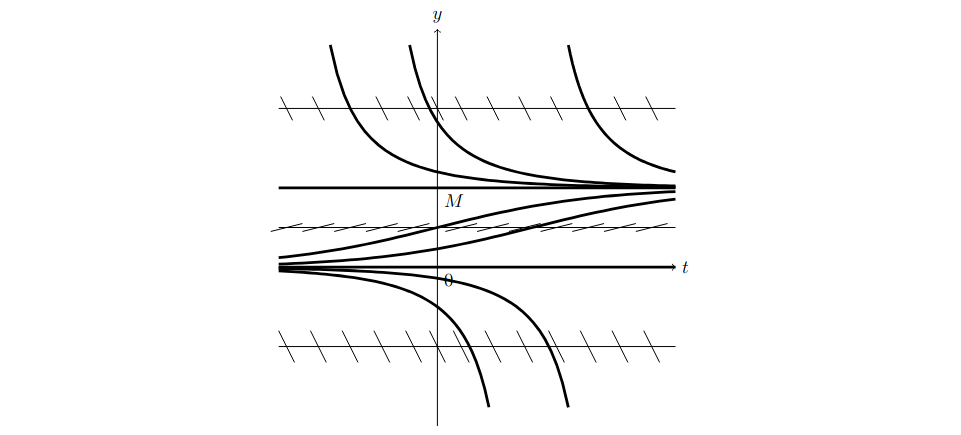
\includegraphics[width=10cm]{16}\\
\end{center}
See that
\begin{enumerate}
\item Since the isoclines are constant in the $t$ direction any solution curve can be translated left or right and 
still be a solution---time invariance.
\item Since the lines $y=0$ and $y=M$ are solutions the other curves can't cross them.
\item The solutions that start above $y=0$ must increase, and since they can't cross $y=M$ they 
tend toward it asymptotically. These bounded solutions
are called \textit{logistic curves}. They represent small populations increasing to $M$.
\item If the population exceeds $M$, they tend back towards it. This represents overpopulation. M is called the 
\textit{carrying capacity} of the environment.
\item Although it doesn't make sense to model a negative numbered population $y<0$, mathematically the solution
curves that start below $y=0$ decrease without bound.
\end{enumerate}
\end{figure}\\
\textbf{Stable and Unstable Equilibria}\\
See that solution curves near the equilibrium $y=M$ tend asymptotically towards it; this is called a 
\textit{stable equilibrium}. Solution curves near the other equilibrium $y=0$ tend away from it; this is called
an \textit{unstable equilibrium}.
\newpage

\subsection{Phase lines, Semistable equilibria}
\textit{Phase lines} allows for the essential content of an autonomous DE:
\begin{equation*}
\dot{y}=f(y)
\end{equation*}
to be conveyed more efficiently. A phase line is drawn using the following steps:
\begin{enumerate}
\item Draw the $y$-axis as a vertical line and mark on it the equilibria---where $f(y)=0$.
\item In each of the intervals delimited by the equilibria draw an upward pointing arrow if $f(y)>0$ and a downward arrow if $f(y)<0$.
\end{enumerate}
Phase lines tells us roughly how the system behaves, capturing the information of a qualitative sketch. Consider 
the following examples.\\
\vspace{1mm}\\
\textbf{Example 1:}\\
Consider the simple autonomous equation
\begin{equation*}
\dot{y}=3y
\end{equation*}
1) First we find the critical points; see that only one critical point exists: $y=0$. 
2) Next we plot the graph of $f(y)$ (in this case a straight line); see that $\dot{y}>0$ for $y>0$ and $\dot{y}<0$ for $y<0$:
\begin{figure}[h]
\begin{center}
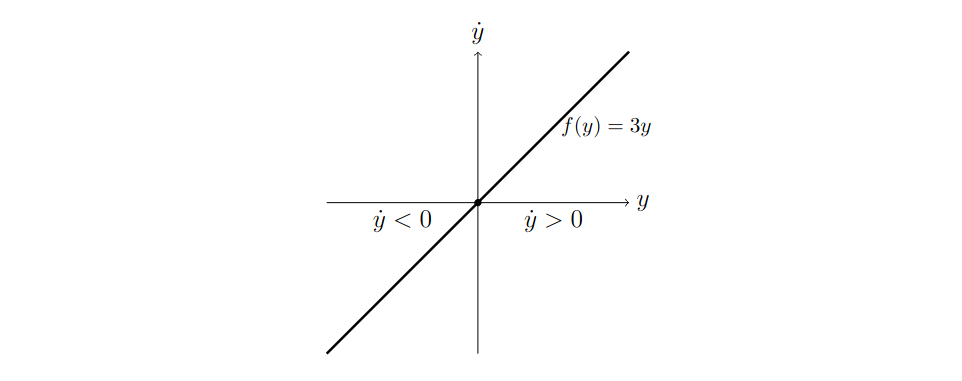
\includegraphics[width=10cm]{17}\\
\end{center}
\end{figure}\\
(next page)
\newpage
\noindent\textbf{Example 1 (cont.)}\\
3) With this we can draw the phase line as outlined above. Since the arrows on the phase line point
away from the critical point, the equilibrium is \textit{unstable}:
\begin{figure}[h]
\begin{center}
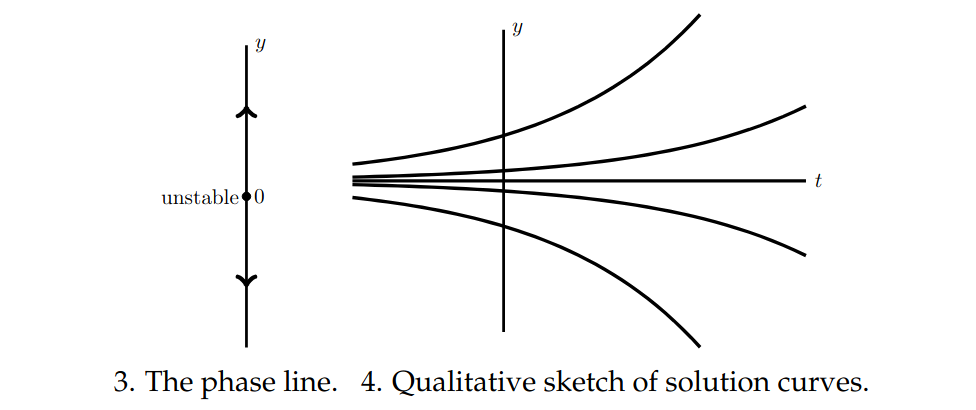
\includegraphics[width=10cm]{18}\\
\end{center}
4) See how the phase line conveys qualitiative information. The equilibrium solution corresponds to the critical
point.
\end{figure}\\
\textbf{Example 2: Logistic equation}\\
Now consider the same solution for the logistic equation:
\begin{figure}[h]
\begin{equation*}
\dot{y}=k_0(1-y/M)y
\end{equation*}
With critical points $y=0,y=M$:
\begin{center}
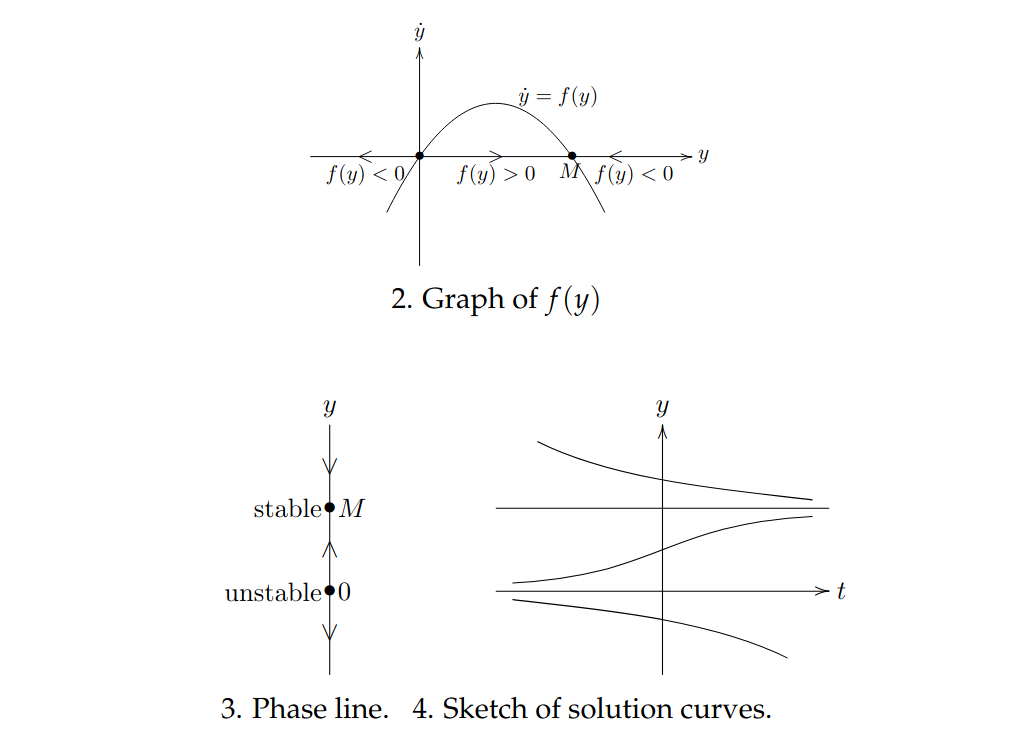
\includegraphics[width=9cm]{19}\\
\end{center}
\end{figure}\\
(next page)
\newpage
\noindent\textbf{Semistable Equilibria}\\
Some equilibria are stable on one side and unstable on the other. We call them \textit{semistable}. 
Consider the DE
\begin{equation*}
\dot{y}=y^2
\end{equation*}
With only one critical point $y=0$:
\begin{figure}[h]
\begin{center}
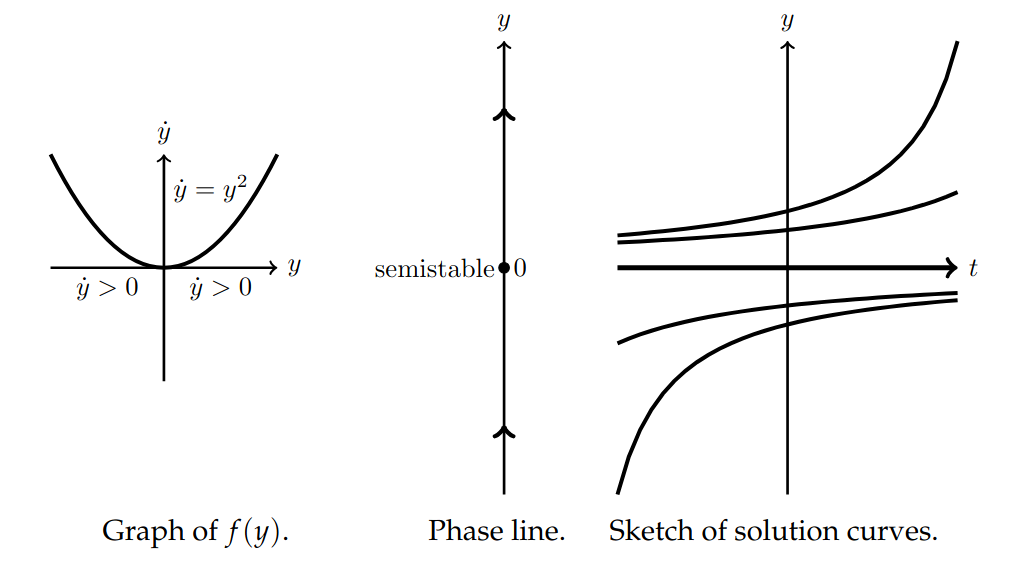
\includegraphics[width=10cm]{20}\\
\end{center}
\end{figure}
\newpage

\section{Second Order Constant Coefficient Linear Equations}
\subsection{Second Order Physical systems---\\Spring-Mass-Dashpot}
\textbf{Spring and Mass}\\
Here we model a second order differential equation. Consider a spring attached to a wall and a cart:
\begin{figure}[h]
\begin{center}
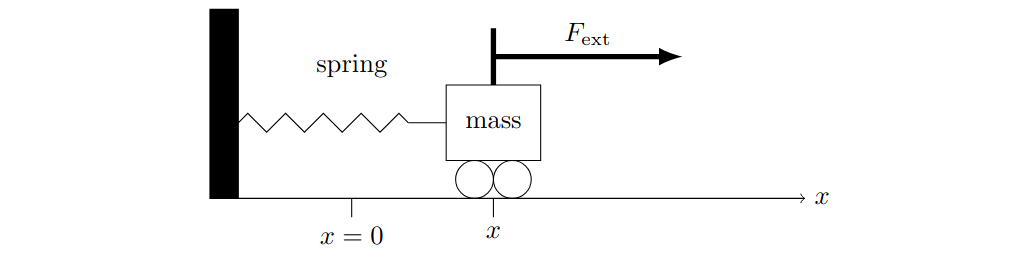
\includegraphics[width=10cm]{21}\\
\end{center}
Consider the coordinate system set in a way that at $x=0$ the spring doesn't exert any force---the equilibrium 
position. Now also consider an external force acting on the mass, the system can be modelled as
\begin{equation*}
m\ddot{x}=F_\text{spr}+F_\text{ext}
\end{equation*}
The spring's behaviour can be characterised by the fact that it depends on the deviation from equilibrium position,
meaning
\begin{align*}
\text{if }x>0,\quad&F_\text{spr}(x)<0\\
\text{if }x=0,\quad&F_\text{spr}(x)=0\\
\text{if }x<0,\quad&F_\text{spr}(x)>0
\end{align*}
The simplest way to model the force exerted by the spring (which is valid in general for small $x$) is
\begin{equation*}
F_\text{spr}(x)=-kx,\text{ where }k>0
\end{equation*}
This is called \textit{Hooke's law}, and $k$ is called the \textit{spring constant}.
\end{figure}\\
Replacing $F_\text{spr}$ by $-kx$ we get
\begin{equation*}
m\ddot{x}+kx=F_\text{ext}
\end{equation*}
(next page)
\newpage
\noindent\textbf{Dashpot}\\
Any real mechanical system has friction, which can take many forms; it is characterised by the fact that it
depends on the motion of the mass. We will suppose that
it depends only on the velocity of the mass and not on its
position.\\
\vspace{1mm}\\
Often dampening is controlled by a device called
the \textit{dashpot} (its a cylinder filled with oil that a piston moves through):
\begin{figure}[h]
\begin{center}
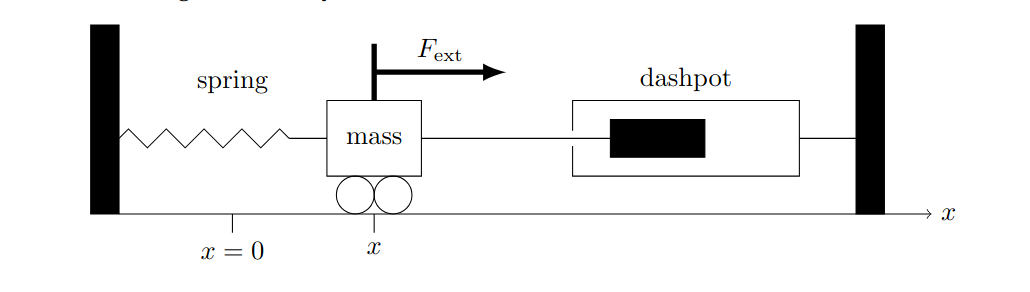
\includegraphics[width=10cm]{22}\\
\end{center}
We write $F_\text{dash}(\dot{x})$ for the force exerted by the dashpot. It opposes the velocity:
\begin{align*}
\text{if }\dot{x}>0,\quad&F_\text{dash}(\dot{x})<0\\
\text{if }\dot{x}=0,\quad&F_\text{dash}(\dot{x})=0\\
\text{if }\dot{x}<0,\quad&F_\text{dash}(\dot{x})>0
\end{align*}
The simplest way to model this (which is also valid for small $\dot{x}$) is
\begin{equation*}
F_\text{dash}(\dot{x})=-b\dot{x},\text{ where }b>0
\end{equation*}
This is called \textit{linear damping}, and $b$ is called the \textit{damping constant}.
\end{figure}\\
Putting this together
\begin{equation*}
m\ddot{x}=F_\text{spr}+F_\text{dash}+F_\text{ext}
\end{equation*}
we get the differential equation for the displacement $x$ of the mass from equilibrium as
\begin{equation*}
m\ddot{x}+b\dot{x}+kx=F_\text{ext}
\end{equation*}
\newpage

\subsection{Linear DEs---Notation}
A \textit{linear differential equation} is of the following form:
\begin{equation*}
a_nx^{(n)}+a_{n-1}x^{(n-1)}+\cdots+a_1\dot{x}+a_0x=q(t)
\end{equation*}
The $a_k$ are the \textit{coefficients}; they may depend on $t$. If $a_n$ is not
zero then the differential equation is said to be of order $n$.\\
\vspace{1mm}\\
If the $a_k$ are constant then the equation is said to be a \textit{constant coefficient linear equation}.

\subsection{Second order homogeneous constant coefficient\\linear equations---Spring system, 
Simple harmonic oscillator}
Consider the spring system in the case where $F_\text{ext}=0$:
\begin{equation*}
m\ddot{x}+b\dot{x}+kx=0
\end{equation*}
With no external force the equation is \textit{homogeneous}.\\
\vspace{1mm}\\
\textbf{Undamped case: Simple harmonic oscillator}\\
The special case where $b=0$ (no dashpot) is called \textit{undamped}. This is called the \textit{simple harmonic
oscillator}.  We can write its ODE as
\begin{equation*}
\ddot{x}+\frac{k}{m}x=0
\end{equation*}
If we let $\omega=\sqrt{k/m}$ our equation becomes
\begin{equation*}
\ddot{x}+\omega^2x=0
\end{equation*}
See that $x_1(t)=\cos(\omega t)$ and $x_2(t)=\sin(\omega t)$ are solutions to this equation. Since the equation is
linear we can use superposition of solutions to get
the solution
\begin{equation*}
x(t)=a\cos(\omega t)+b\sin(\omega t)=A\cos(\omega t-\phi)
\end{equation*}
This is the \textit{general solution}. We know it gives every solution because
$x(0)=a$ and $\dot{x}(0)=\omega b$---by solving (uniquely) for $a$ and $b$ we can get any desired initial condition.
\newpage

\subsection{Characteristic polynomial}
\textbf{2nd Order Case}\\
For $m,b,k$ constant, consider the homogeneous equation
\begin{equation*}
m\ddot{x}+b\dot{x}+kx=0
\end{equation*}
Consider solutions of the form $x=e^{rt}$. We have
\begin{equation*}
m\ddot{x}+b\dot{x}+kx=(mr^2+br+k)e^{rt}=0
\end{equation*}
Since an exponential is never zero, $e^{rt}$ is therefore a solution exactly when $r$ satisfies the
\textit{characteristic equation} (the left hand side is the \textit{characteristic polynomial}):
\begin{equation*}
mr^2+br+k=0
\end{equation*}
\textbf{Example}\\
Consider the DE
\begin{equation*}
\ddot{x}+8\dot{x}+7x=0
\end{equation*}
The characteristic polynomial here is $r^2+8r+7$. Solving for $r$ by factorisation we have $(r+1)(r+7)$ and 
the roots $r=-1$ and $r=-7$. Therefore the corresponding exponential solutions are
$x_1(t)=e^{-t}$ and $x_2(t)=e^{-7t}$.\\
\vspace{1mm}\\
By superposition, the linear combination of independent solutions gives the general solution:
\begin{equation*}
x(t)=c_1e^{-t}+c_2e^{-7t}
\end{equation*}
Where given initial conditions for $x$ and $\dot{x}$ we can solve for $c_1$ and $c_2$.\\
\vspace{1mm}\\
\textbf{General $n$th Order Case}\\
See that using the same principle we can take the homogeneous constant coefficient linear equation of degree $n$:
\begin{equation*}
a_nx^{(n)}+\cdots+a_1\dot{x}+a_0x=0
\end{equation*}
and get its characteristic polynomial
\begin{equation*}
p(r)=a_nr^n+\cdots+a_1r+a_0
\end{equation*}
In which the exponential $x(t)=e^{rt}$ is a solution of the homogeneous DE if and only if $r$ is a root
of $p(r)$ (meaning $p(r)=0$). By superposition, any linear combination of these exponentials is also a solution.
\newpage

\subsection{Modes and Roots (real and complex)\\(homogeneous constant coefficient linear equations)}
\textbf{Modes}\\
A solution of the form $x(t)=ce^{rt}$ to the homogeneous constant coefficient linear equation:
\begin{equation*}
a_nx^{(n)}+a_{n-1}x^{(n-1)}+\cdots+a_1\dot{x}+a_0x=0
\end{equation*}
is called a \textit{modal solution} and $ce^{rt}$ the \textit{mode} of the system. Recall that
$e^{rt}$ is a solution exactly when $r$ is a root of the characteristic polynomial
\begin{equation*}
p(s)=a_ns^n+a_{n-1}s^{n-1}+\cdots+a_1s+a_0
\end{equation*}
(note this only works for \textit{homogeneous constant coefficient linear equations}; it won't apply to
non-constant coefficient or inhomogeneous or nonlinear equations.)\\
\vspace{1mm}\\
\textbf{Real roots}\\
The roots of these polynomials can be real or complex. Roots can also be repeated. First consider the real case for
a second order homogeneous constant coefficient DE:
if the characteristic polynomial has real roots $r_1$ and $r_2$ then the \textit{modal} solutions are 
$x_1(t)=e^{r_1t}$ and $x_2(t)=e^{r_2t}$. The general solution can be found by superposition:
\begin{equation*}
x(t)=c_1x_1(t)+c_2x_2(t)=c_1e^{r_1t}+c_2e^{r_2t}
\end{equation*}
\textbf{Example}\\
Solving $\ddot{x}+5\dot{x}+4x=0$: The characteristic equation is
\begin{equation*}
s^2+5s+4=(s+1)(s+4)=0
\end{equation*}
Which has roots -1 and -4. The modal solutions are $x_1(t)=e^{-t}$ and $x_2(t)=e^{-4t}$. Therefore
the general solution is
\begin{equation*}
x(t)=c_1e^{-t}+c_2e^{-4t}
\end{equation*}
(next page)
\newpage
\noindent\textbf{Complex roots---illustrative example}\\
Consider now the equation $\ddot{x}+4\dot{x}+5x=0$. The characterisic polynomial is $s^2+4s+5$. 
Using the quadratic formula the roots are
\begin{equation*}
s=\frac{-4\sqrt{16-20}}{2}=-2\pm\sqrt{-1}=-2\pm i
\end{equation*}
So our exponential solutions are (using the letter $z$ to indicate they are complex valued):
\begin{equation*}
z_1(t)=e^{(-2+i)t}\quad\text{and}\quad z_2(t)=e^{(-2-i)t}
\end{equation*}
The DE has real coefficients, we expect \textit{real solutions}. To get them, consider the following theorem:\\
\vspace{1mm}\\
\textbf{Real Solution Theorem:}\\
\textit{Theorem:} If $z(t)$ is a complex-values solution to $m\ddot{z}+b\dot{z}+kz=0$, where $m,b,k$ are real, 
then the real and imaginary parts of $z$ are also solutions.\\
\vspace{1mm}\\
\textit{Proof:} Letting $u(t)$ be the real part of $z$ and $v(t)$ the imaginary part, so that
$z(t)=u(t)+iv(t)$, see that the DE can be written as
\begin{equation*}
(m\ddot{u}+b\dot{u}+ku)+i(m\ddot{v}+b\dot{v}+kv)=0
\end{equation*}
Both expressions in parentheses are real. The only way for the sum to be 0 is if both expressions are 0. 
That is, both $u$ and $v$ are solutions.\\
\vspace{1mm}\\
\textbf{Illustrative example cont.}\\
We had $z_1(t)=e^{(-2+i)t}$ and $z_2(t)=e^{(-2-i)t}$. Using Euler's formula:
\begin{equation*}
z_1(t)=e^{(-2+i)t}=e^{-2t}\cos t+ie^{-2t}\sin t
\end{equation*}
Both the real part $e^{-2t}\cos t$ and imaginary part $e^{-2t}\sin t$ are solutions. We now have two \textit{basic}
solutions and can use superposition to obtain the general
\textit{real valued} solution
\begin{equation*}
x(t)=c_1e^{-2t}\cos(t)+c_2e^{-2t}\sin(t)
\end{equation*}
See that choosing the other exponential solution
\begin{equation*}
z_2(t)=e^{(-2+i)t}=e^{-2t}\cos(-t)+ie^{-2t}\sin(-t)
\end{equation*}
would give the basic real solutions
\begin{equation*}
e^{-2t}\cos(t)\quad\text{and}\quad-e^{-2t}\sin(t)
\end{equation*}
Which would give the same general solution.\\
(next page)
\newpage
\noindent\textbf{More on complex roots}\\
We had the general solution
\begin{equation*}
c_1e^{-2t}\cos(t)+c_2e^{-2t}\sin(t)
\end{equation*}
See that the solution can be written in a different form:
\begin{equation*}
x(t)=e^{-2t}(c_1\cos(t)+c_2\sin(t))=Ae^{-2t}\cos(t-\phi)
\end{equation*}
This is a \textit{damped sinusoid} with \textit{circular pseudo-frequency} 1.\\
\vspace{1mm}\\
\textbf{Example}\\
Solving $\ddot{x}+\dot{x}+x=0$, the characteristic equation is $s^2+s+1=0$ and the roots
\begin{equation*}
\frac{-1\pm\sqrt{1-4}}{2}=\frac{-1}{2}\pm i\frac{\sqrt{3}}{2}
\end{equation*}
We have the complex exponential solutions
\begin{equation*}
z_1(t)=e^{(-1+i\sqrt{3})t/2},\quad z_2(t)=e^{(-1-i\sqrt{3})t/2} 
\end{equation*}
From this we obtain the basic real solutions
\begin{equation*}
\text{Re}(z_1(t))=e^{-t/2}\cos(\sqrt{3}t/2),\quad
\text{Im}(z_1(t))=e^{-t/2}\sin(\sqrt{3}t/2)
\end{equation*}
and therefore the general real solution
\begin{equation*}
e^{-t/2}(c_1\cos(\sqrt{3}t/2)+c_2\sin(\sqrt{3}t/2))
=Ae^{-t/2}\cos(\sqrt{3}t/2-\phi)
\end{equation*}
\textbf{In general}\\
In general, supposing the equation $m\ddot{x}+b\dot{x}+kx=0$ has the characteristic roots
$a\pm ib$, two real solutions are
\begin{equation*}
e^{at}\cos(bt)\quad\text{and}\quad e^{at}\sin(bt)
\end{equation*}
and the general real solution is
\begin{equation*}
c_1e^{at}\cos(bt)+c_2e^{at}\sin(bt)=Ae^{at}\cos(bt-\phi)
\end{equation*}
\newpage

\subsection{Repeated roots\\(homogeneous constant coefficient linear equations)}
\textbf{Illustrative example}\\
Consider $\ddot{x}+4\dot{x}+4x=0$. In this case the
characteristic equation:
\begin{equation*}
P(s)=s^2+4s+4=(s+2)^2
\end{equation*}
has $r=-2$ as a repeated root. The only exponential solution is $e^{-2}t$. 
To get the second basic exponential solution, see that
$te^{-2t}$ is also a solution. Our general solution is 
therefore
\begin{equation*}
x(t)=c_1e^{-2t}+c_2te^{-2t}
\end{equation*}
\textbf{Deriving solution for second order repeated roots}\\
Considering the DE $a\ddot{x}+b\dot{x}+cx=0$, from the characteristic equation we know
\begin{equation*}
r_{1,2}=\frac{-b\pm\sqrt{b^2-4ac}}{2a}
\end{equation*}
Should we only have one solution, as per the quadratic formula, we must have
\begin{equation*}
b^2-4ac=0,\quad\text{and}\quad r_{1,2}=-\frac{b}{2a}
\end{equation*}
We know one solution is $x_1=e^{-b/(2a)t}$. Consider a second solution of the form 
\begin{equation*}
x_2=v(t)x_1
\end{equation*}
we want to plug $x_2$ into the DE. For that we require its derivatives:
\begin{align*}
x_2'&=v'e^{-b/(2a)t}-\frac{b}{2a}ve^{-b/(2a)t}\\
x_2''&=v''e^{-b/(2a)t}-\frac{b}{2a}v'e^{-b/(2a)t}
-\frac{b}{2a}v'e^{-b/(2a)t}+\frac{b^2}{4a^2}ve^{-b/(2a)t}
\\&=v''e^{-b/(2a)t}-\frac{b}{a}v'e^{-b/(2a)t}+\frac{b^2}{4a^2}ve^{-b/(2a)t}
\end{align*}
Evaluating the DE with our proposed solution $x_2$:
\begin{align*}
a\left(v''e^{-b/(2a)t}-\frac{b}{a}v'e^{-b/(2a)t}+\frac{b^2}{4a^2}ve^{-b/(2a)t}\right)&+\\
b\left(v'e^{-b/(2a)t}-\frac{b}{2a}ve^{-b/(2a)t}\right)
&+c\left(ve^{-b/(2a)t}\right)=0
\end{align*}
Factoring out the exponential we get
\begin{align*}
&e^{-b/(2a)t}\left(av''-bv'+\frac{b^2}{4a}v+bv'-\frac{b^2}{2a}v+cv\right)\\
&=e^{-b/(2a)t}\left(av''+\left(-\frac{b^2}{4a}+c\right)v\right)\\
&=e^{-b/(2a)t}\left(av''-\frac{1}{4a}\left(b^2-4ac\right)v\right)=0
\end{align*}
(next page)
\newpage
\noindent\textbf{Derivation continued}\\ 
Evaluating the DE with our proposed solution $x_2=ve^{-b/(2a)t}$ gave us
\begin{equation*}
e^{-b/(2a)t}\left(av''-\frac{1}{4a}\left(b^2-4ac\right)v\right)=0
\end{equation*}
We know that $b^2-4ac=0$ (since the quadratic equation only has one solution as mentioned before). Thus since
exponentials cannot be zero, we have 
\begin{equation*}
av''=0\implies v''=0
\end{equation*}
(since $a\neq0$.) We can then determine $v(t)$:
\begin{equation*}
v'=\int v''dt=k\implies v=\int v'dt=k_1t+k_2
\end{equation*}
We therefore have our proposed basic solutions as
\begin{equation*}
x_1=e^{-b/(2a)t},\quad x_2=vx_1=(k_1t+k_2)e^{-b/(2a)t}
\end{equation*}
see that combining our solutions into a general solution via superposition gives
\begin{equation*}
x(t)=c_1e^{-b/(2a)t}+c_2(k_1t+k_2)e^{-b/(2a)t}
\end{equation*}
See that this can be simplified since $c_1,c_2,k_1,k_2$ are all unknown constants
\begin{equation*}
x(t)=(c_1+c_2k_2)e^{-b/(2a)t}+c_2k_1te^{-b/(2a)t}
\end{equation*}
We have
\begin{equation*}
x(t)=C_1e^{-b/(2a)t}+C_2te^{-b/(2a)t}
\end{equation*}
See that since we are dealing with a homogeneous equation,
$te^{-b/(2a)t}$ by itself satisfies the DE (because of superposition).
\newpage

\subsection{Damped harmonic oscillators}
\textbf{Spring-mass-dashpot}\\
Recall the model spring-mass-dashpot system with the constant coefficient linear DE:
\begin{figure}[h]
\begin{equation*}
m\ddot{x}+b\dot{x}+kx=F_\text{ext}
\end{equation*}
where $m$ is the mass, $b$ the damping constant, $k$ the spring constant, and $x(t)$ the displacement
of the mass from its equilibrium position.
\begin{center}
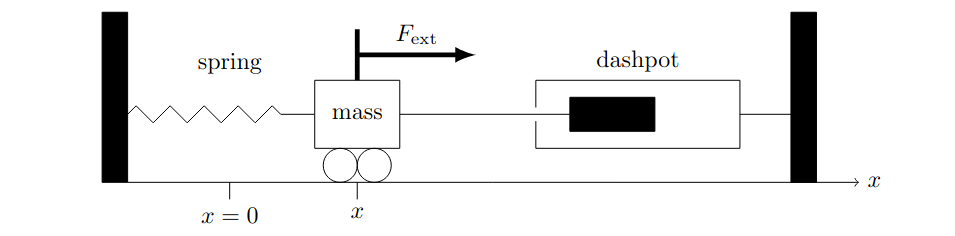
\includegraphics[width=10cm]{23}\\
\end{center}
Assuming zero external force ($F_\text{ext}=0$), we have
the homogeneous equation
\begin{equation*}
m\ddot{x}+b\dot{x}+kx=0
\end{equation*}
The algebra doesn't require any restrictions on $m,b,k$, except $m\neq0$ (for the equation to be second order
in the first place). But in this physical model we require $m>0,b\geq0$, and $k>0$.
\end{figure}\\
(next page)
\newpage
\noindent\textbf{Damped harmonic oscillator}
\begin{figure}[h]
The \textit{undamped} ($b=0$) system has the equation
\begin{equation*}
m\ddot{x}+kx=0
\end{equation*}
We have its solution as
\begin{equation*}
x(t)=c_1\cos(\omega t)+c_2\sin(\omega t)=A\cos(\omega t-\phi)
\end{equation*}
Here $\omega=\sqrt{k/m}$. The solution is always a sinusoid, thus we call this a 
\textit{simple harmonic oscillator}:
\begin{center}
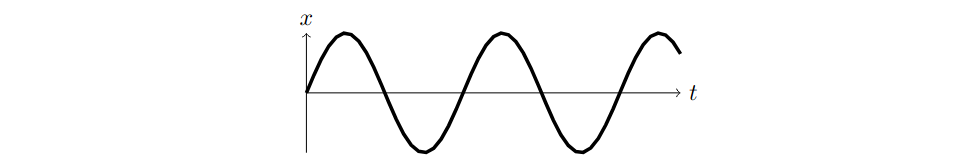
\includegraphics[width=10cm]{24}\\
\end{center}
When we add damping ($b>0$) we then call the system a \textit{damped harmonic oscillator}.\\
\vspace{1mm}\\
This emphasises an important fact about uding DEs to model physical systems:
Any system modeled by the same equation will respond just like the spring-mass-dashpot (regardless of what $m,d,k,x$
represent). That is, all damped harmonic oscillators exhibit similar behaviour.
\end{figure}
\newpage

\subsection{Under, Over and Critical damping}
\textbf{Response to damping}\\
As we saw, the unforced damped harmonic oscillator has equation
\begin{equation*}
m\ddot{x}+b\dot{x}+kx=0
\end{equation*}
with $m>0,b\geq0$ and $k>0$. It has characteristic equation
\begin{equation*}
ms^2+bs+k=0
\end{equation*}
with characteristic roots
\begin{equation*}
\frac{-b\pm\sqrt{b^2-4mk}}{2m}
\end{equation*}
There are three cases depending on the sign of the expression under the square root:
\begin{enumerate}
\item $b^2<4mk$---\textit{Underdamping}
\item $b^2>4mk$---\textit{Overdamping}
\item $b^2=4mk$---\textit{Critical damping}
\end{enumerate}
\textbf{First case: Underdamping}\\
If $b^2<4mk$ the square root is negative and the characteristic roots are complex. See that the roots are given by
\begin{equation*}
-\frac{b}{2m}\pm i\omega_d,\quad\text{where }\omega_d=\frac{\sqrt{|b^2-4mk|}}{2m}
\end{equation*}
With that we have the complex exponential solutions
\begin{equation*}
e^{(-b/(2m)+i\omega_d)t},\quad e^{(-b/(2m)-i\omega_d)t}
\end{equation*}
With the basic real solutions
\begin{equation*}
e^{-bt/(2m)}\cos(\omega_dt),\quad e^{-bt/(2m)}\sin(\omega_dt)
\end{equation*}
The general real solution is found by taking linear combinations of two basic solutions:
\begin{equation*}
x(t)=c_1e^{-bt/(2m)}\cos(\omega_dt)+c_2e^{-bt/(2m)}\sin(\omega_dt)
\end{equation*}
This can also be written as
\begin{equation*}
x(t)=e^{-bt/(2m)}(c_1\cos(\omega_dt)+c_2\sin(\omega_dt))
=Ae^{-bt/(2m)}\cos(\omega_dt-\phi)
\end{equation*}
(next page)
\newpage
\noindent\textbf{Underdamping---Intuition}\\
We had the behaviour of an underdamped system as
\begin{equation*}
Ae^{-bt/(2m)}\cos(\omega_dt-\phi)
\end{equation*}






\newpage

\subsection{Superposition (Second order ODEs)}%100524--\underbrace, \quad, align, \left[\right]
The Principle of Superposition for Second Order Differential Equations; if
\begin{equation*}
\frac{d^2y}{dt^2}+p(t)\frac{dy}{dt}+q(t)y=0
\end{equation*}
is a second order linear differential equation and $y=y_1(t)$ and $y=y_2(t)$ are both
solutions to this differential equation, then for $C$ and $D$ as constants,
\begin{equation*}
y=Cy_1(t)+Dy_2(t)\quad\text{is also a solution}
\end{equation*}
Essentially, any linear combination of solutions is also a solution.\\
\vspace{1mm}\\
\textit{Proof}: Consider $y=y_1$ and $y=y_2$ are solutions to the second
order linear differential equation $\frac{d^2y}{dt^2}+p(t)\frac{dy}{dt}+q(t)y=0$. Then we have
that:
\begin{equation*}
\frac{d^2y_1}{dt^2}+p(t)\frac{dy_1}{dt}+q(t)y_1=0\quad\text{and}\quad\frac{d^2y_2}{dt^2}+p(t)\frac{dy_2}{dt}+q(t)y_2=0
\end{equation*}
If $C$ and $D$ are constants, plugging in $y=Cy_1(t)+Dy_2(t)$:
\begin{align*}
&\frac{d^2}{dt^2}(Cy_1(t)+Dy_2(t))+p(t)\frac{d}{dt}(Cy_1(t)+Dy_2(t))
+q(t)(Cy_1(t)+Dy_2(t))\\
&=C\frac{d^2y_1}{dt^2}+D\frac{d^2y_2}{dt^2}+p(t)C\frac{dy_1}{dt}+p(t)D\frac{dy_2}{dt}
+q(t)Cy_1+q(t)Dy_2\\
&=C\underbrace{\left[\frac{d^2y_1}{dt^2}+p(t)\frac{dy_1}{dt}+q(t)y_1\right]}_{=0}
+D\underbrace{\left[\frac{d^2y_2}{dt^2}+p(t)\frac{dy_2}{dt}+q(t)y_2\right]}_{=0}\\
&=0
\end{align*}
Therefore, $y=Cy_1(t)+Dy_2(t)$ is also a solution. Note that the superposition principle
\textbf{does not} work for nonlinear differential equations.\\
(next page)
\newpage
\noindent\textbf{In context of inhomogenous differential equations}\\ %120524 \textit{}, \textbf{}
In addition, if $y_1$ is a solution to:
\begin{equation*}
\frac{d^2y}{dt^2}+p(t)\frac{dy}{dt}+q(t)y=f_1(t)
\end{equation*}
and $y_2$ is a solution to:
\begin{equation*}
\frac{d^2y}{dt^2}+p(t)\frac{dy}{dt}+q(t)y=f_2(t)
\end{equation*}
then for constants $C$ and $D$, $Cy_1+Dy_2$ is a solution to:
\begin{equation*}
\frac{d^2y}{dt^2}+p(t)\frac{dy}{dt}+q(t)y=Cf_1(t)+Df_2(t)
\end{equation*}
\textit{Proof}: Plugging in $y=Cy_1+Dy_2$:
\begin{align*}
&\frac{d^2}{dt^2}(Cy_1+Dy_2)+p(t)\frac{d}{dt}(Cy_1+Dy_2)+q(t)(Cy_1+Dy_2) \\
&=C\frac{d^2y_1}{dt^2}+D\frac{d^2y_2}{dt^2}+p(t)C\frac{dy_1}{dt}+p(t)D\frac{dy_2}{dt}
+q(t)Cy_1+q(t)Dy_2\\
&=C\underbrace{\left[\frac{d^2y_1}{dt^2}+p(t)\frac{dy_1}{dt}+q(t)y_1\right]}_{=f_1(t)}
+D\underbrace{\left[\frac{d^2y_2}{dt^2}+p(t)\frac{dy_2}{dt}+q(t)y_2\right]}_{=f_2(t)}\\
&=Cf_1(t)+Df_2(t)
\end{align*}
Superposition is therefore \textit{not} limited to homogenous equations.

\subsection{General solution for inhomogenous linear ODEs} %120524
Therefore, to get the general solution $y(t)$ to an inhomogenous linear ODE:
\begin{align*}
\text{inhomogenous:}\quad\frac{d^2y}{dt^2}+p(t)\frac{dy}{dt}+q(t)y=f(t)
\end{align*}
1. Find the general solution $y_h$ to the associated \textbf{homogenous} equation:
\begin{align*}
\text{homogenous:}\quad\frac{d^2y_h}{dt^2}+p(t)\frac{dy_h}{dt}+q(t)y_h=0
\end{align*}
2. Find (in some way) any \textbf{one particular solution} $y_p$ to the \textbf{inhomogenous} ODE.
\\
3. Add $y_p$ to $y_h$ to get the general solution to the inhomogenous ODE:
\begin{align*}
\underbrace{y}_{\text{general \textbf{inhomogenous} solution}}=
\underbrace{y_p}_{\text{\textbf{any particular solution}}}+
\underbrace{y_h}_{\text{general \textbf{homogenous} solution}}
\end{align*}
Note that the superposition principle \textbf{does not} work for nonlinear differential equations.

\subsection{Existence and uniqueness} %130524 \vspace{}
Solving a first-order linear ODE leads to a 1-parameter family of solutions (a general solution).
To derive a specific solution, we need an initial condition, such as $y(0)$. One may wonder if
there are other solutions. Here is a general result which says that there aren't and confirms 
that our methods find all solutions:\\
\vspace{2mm}\\
\textbf{Existence and uniqueness theorem for a linear ODE:}\\
Let $p(t)$ and $q(t)$ be continuous functions on an open interval $I$. Let $a\in I$, and let $b$
be a given number. Then there \textbf{exists} a \textbf{unique} solution defined on the entire 
interval $I$ to the first order linear ODE
\begin{equation*}
\dot{y}+p(t)y=q(t)
\end{equation*}
satisfying the initial condition
\begin{equation*}
y(a)=b
\end{equation*}
\textbf{Existence} means there is \textbf{at least one} solution.\\
\textbf{Uniqueness} means that there is \textbf{only one} solution.

\subsection{Exponential response formula}
The exponential response formula gives us a quick method for finding the particular solution to 
any linear, constant coefficient, differential equations whose input can be expressed in terms
of an exponential function.\\
\vspace{2mm}\\
The Exponential Response Formula(ERF): 

\section{Fourier Series}
\subsection{Fourier Series}
If the input function $f(t)$ is periodic (of period $2\pi$)
,we can express the function (where it is continuous) as an
infinite sum of sines and cosines.
This series representation is called a Fourier Series:
\begin{align*}
f(t)&=c_0+\sum_{n=1}^{\infty}[a_n\cos(nt)+b_n\sin(nt)], 
& \text{$c_0, a_n, b_n$ real constants}
\end{align*}




















\end{document}

